%  --------------------- chapter 3--------------------- %
\chapter{大气运动驱动力变化对陆地地表风速长期变化的影响}\label{chap:drivingforceonwind}

\section{引言}

第\ref{chap:SpatiotemporalCharacteristics}章全面分析了北半球陆地地表风速长期变化的时空特征,从本章开始探讨其背后的原因。如第一章所述,风速变化究其根本可以从大气运动驱动力的变化和大气运动阻力的变化两个方面来解释,本章将重点分析大气运动驱动力变化的影响。

垂直方向上来看,西风带大气运动的动量从高层向低层传递,并在地面被摩擦作用消耗掉。因此,了解高层大气风速变化对理解地表风速变化的原因非常重要。之前少有研究涉及风速的垂直变化,\citet{vautard2010northern}发现1979-2008年间北半球高层风速没有出现像地表风速一样的普遍减弱的情况,\citet{lin2013observed}发现1960-2009年间中国高层风速与地表风速变化存在一定的相似性,因而地表风速变化可以一定程度上由高层变化解释。本章将首先全面分析北半球自由大气各个层次的长期变化特征以及它们与地表风速长期变化的区别和联系。

气压场的变化与大气运动驱动力变化直接相关。\citet{zhang2019increase}利用简化的动力学模型分析发现海平面气压场变化是1970年以来北半球陆地地表风速月变化的主导因素,\citet{wu2016estimating}发现海平面气压场可以很大程度上解释中国东部地区陆地地表风速的季节和年际变率。本章对全球冬季和夏季的海平面气压场长期趋势进行了分析,探究大尺度气压场变化对于陆地地表风速的影响。

环流系统的变化是大气运动驱动力变化的重要反映,大尺度海温同样会影响大气驱动力,而环流系统与大尺度海温两者的变化又通常相互联系。例如,NAO的定义为500hPa位势高度场进行旋转经验正交分解(REOF)的第一模态,反映的是冰岛低压和亚速尔高压的强弱交替如跷跷板一般的变化\citep{wallace1981teleconnections}。诸多研究表明,NAO变率可以对欧洲地表风速产生显著影响\citep{beniston2005mountain, earl20131980–2010},同时,NAO变率受到大西洋海温的影响\citep{frankignoul2005observed}。与NAO类似,AO的变率也会影响大尺度陆地地表风速\citep{chen2013wind},也与海温有一定联系\citep{yasunaka2002regime}。大尺度海温模态太平洋年代际振荡(PDO)也被认为与大尺度陆地地表风速变化有一定联系\citep{fu2011temporal}。本章同样分析了环流系统及大尺度海温变化对于北半球陆地地表风速的影响。

\section{资料和方法}

本章研究使用了以下数据集:

IGRA V2全球探空数据集\citep{durre2006overview}由NOAA制作,包含全球超过2700个探空站点的观测数据。此数据集进行了一系列质量控制,对可疑和错误数据进行了标记。本章研究选取了1979-2016年850 hPa、700 hPa、500 hPa和200 hPa风速数据进行分析。为了保证数据质量,剔除了所有被标记为可疑和错误的数据;剔除了1981年1月的所有数据,因为此时间段数据有较大问题\citep{vautard2010northern};若某站点在某年内在某个层次任意一个季节内有记录天数少于45天,则移除此站点当年在此层次所有数据,若此站点在此层次有记录年数少于20年,则移除此层次所有数据。经过质量控制后,850 hPa、700 hPa、500 hPa和200 hPa分别剩余558、578、559和527个站点。本章中对流层风速相关分析均是基于此数据集。

\href{https://b2share.eudat.eu/records/159158152f4d4be79559e2f3f6b1a410}{高塔观测数据集}由巴塞罗那超算中心(BSC)制作,包含全球183个观测塔数据。此数据集针对风速进行了18项数据质量检测,删除了错误数据。此数据集中包含的观测序列大多时间较短,在北美洲仅有5个站点有30年以上的观测长度,因而选择此5个站点分析地表以上30 - 50 m高度风速变化。由于此5个站点均不包含10 m标准高度的风速观测,因而选取HadISD v3(\citet{dunn2012hadisd:},此数据集由第二章使用到的NCEI-ISD整理而成,不同于NCEI-ISD以时间为单位存储,即每月的数据存储在一个文件中,此套数据以站点为单位存储,即每个站点的数据存储在一个文件中,更易于少量站点数据的读取)中与它们距离最近的站点风速进行对比。

HadSLP2r全球海平面气压观测数据集\citep{allan2006a}由哈德莱中心(Hadley Centre)制作,包含1850年至今全球海平面气压场数据。此数据集使用ICOADS海洋观测数据和2228个陆地观测站数据,最终制作成$5 \times 5$度格点数据,并由NOAA PSD转换成NetCDF格式提供\href{https://www.esrl.noaa.gov/psd/gcos_wgsp/Gridded/data.hadslp2.html}{下载} 。此套数据进行了一系列质量控制减少人为误差造成的影响。本章使用此数据集1979-2016年数据分析全球海平面气压场的长期趋势。

HadSST3全球海表温度观测数据集\citep{kennedy2011reassessing1,kennedy2011reassessing2}由哈德莱中心制作,包含1850年至今全球海表温度。此数据集使用ICOADS、GST和ERDDAP海洋观测数据,制作成$5 \times 5$度格点数据。此数据集进行了一系列质量控制减少人为误差造成的影响。本章使用此数据集1979-2016年数据分析其与陆地地表风速序列的相关性。

中国气象局国家气候中心\href{https://cmdp.ncc-cma.net/Monitoring/cn_index_130.php}{百项气候系统指数集}整理了130项大气环流、海温和其他指数,其中涵盖了厄尔尼诺-南方涛动(ENSO),NAO、AO、PDO等环流和海温指数。经过检查,发现其中AO指数与其他研究存在较大差别,因而没有使用,转而使用NOAA计算的\href{https://www.ncdc.noaa.gov/teleconnections/ao/}{AO指数}。本章中使用这些环流和海温指数与陆地地表风速进行对比,以找出它们之间的联系。

本章中计算线性趋势和统计显著性检验的方法与第二章相同。相关系数计算使用Pearson相关系数,计算方法如下:

\begin{equation} \label{eq:pearsoncorr}
r = \frac{cov \left(A, ~ B \right)}{\sigma_{A}\sigma_{B}}
\end{equation} ~\\
其中,$cov \left(A, ~ B \right)$为序列$A$、$B$的协方差,$\sigma_{A}$、$\sigma_{B}$分别为$A$、$B$的标准差。

\section{对流层风速长期变化}

\subsection{对流层风速长期线性趋势}

\begin{figure}[!htbp]
    \centering
    \includegraphics[width=0.75\textwidth]{对流层风速趋势}
    \bicaption{对流层风速趋势($m ~ s^{-1}$每十年)。a)200 hPa,b)500 hPa,c)700 hPa,d)850 hPa,e)地面。}{Troposphere wind speed trends (in $m ~ s^{-1} ~ decade^{-1}$). a)200 hPa, b)500 hPa, c)600 hPa, d)850 hPa, e)Surface.}
    \label{fig:tropospherewindtrend}
\end{figure}

\begin{figure}[!b]
    \centering
    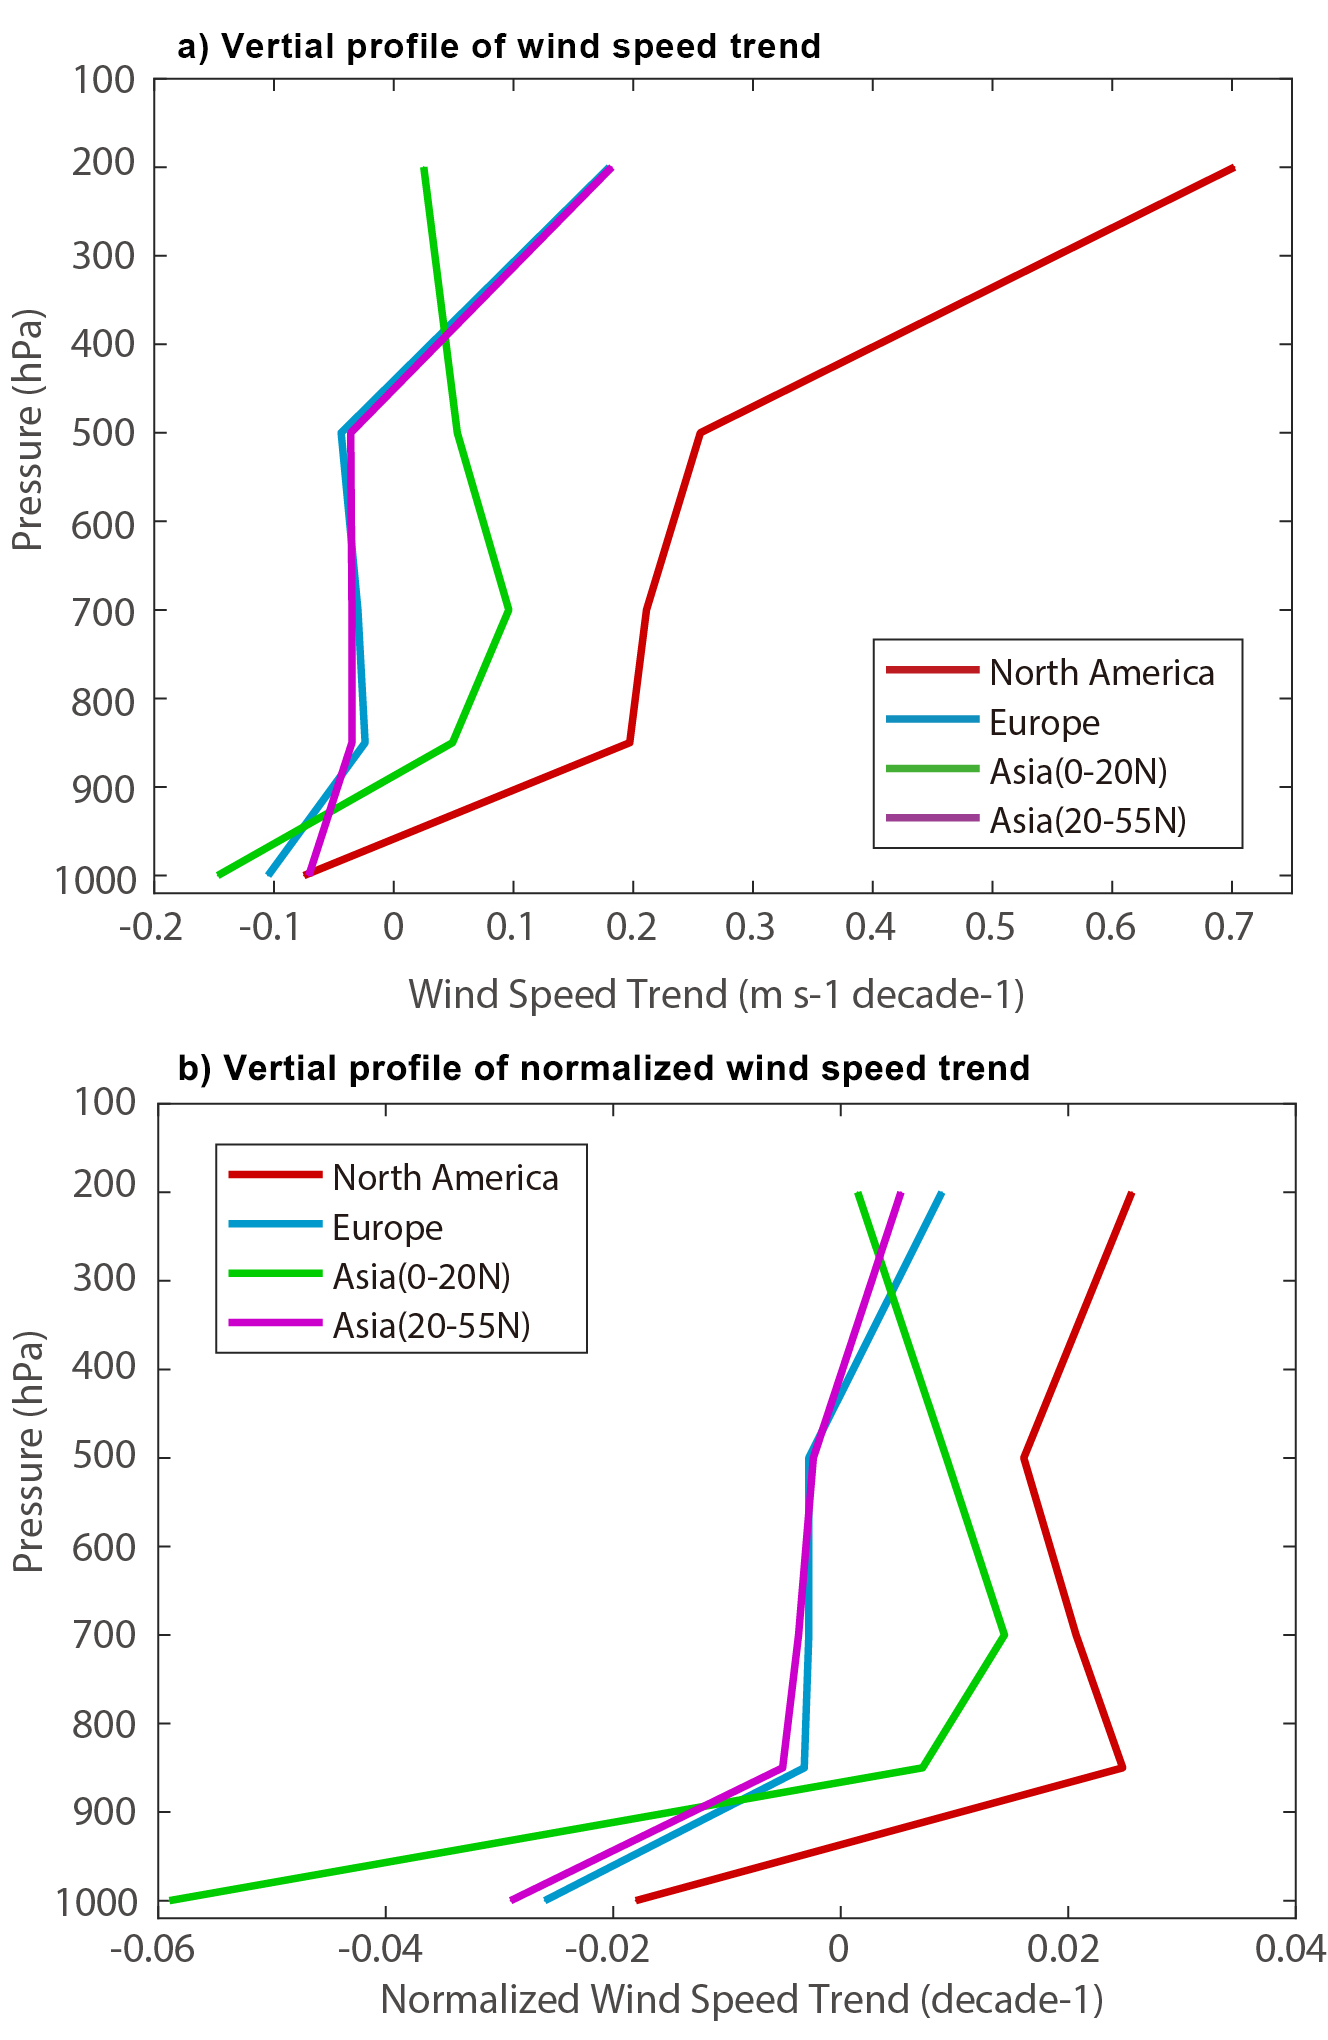
\includegraphics[width=0.65\textwidth]{对流层中位数风速趋势}
    \bicaption{对流层中位数风速趋势($m ~ s^{-1}$每十年)。a)原始风速趋势,b)归一化风速趋势,即原始风速趋势/平均风速。红线为北美洲,蓝线为欧洲,绿线为亚洲低纬度地区(0-20 N),紫线为亚洲中纬度地区(20-55 N)。}{Troposphere median wind speed trends (in $m ~ s^{-1} ~ decade^{-1}$). a) Original wind speed trends. b) Normalized wind speed trends, i.e. original wind speed trends divided by climatological wind speed. Red line denotes North America, blue denotes Europe, green denotes Asian low altitude area (0-20 N), purple denotes Asian mid-latitude area (20-55 N). }
    \label{fig:tropospheremedianwindtrend}
\end{figure}


使用IGRA V2探空风速数据计算了对流层850 hPa、700 hPa、500 hPa和200 hPa长期趋势,分别代表对流层低层、中低层、中层和高层的状况,发现风速的长期趋势在垂直方向上有很大的不均匀性,地表风速减弱最为剧烈,而对流层风速有微弱减小甚至增加(图 \ref{fig:tropospheremedianwindtrend})。在北美洲,地表风速普遍减小,而自由大气风速在各个层次均出现上升(图 \ref{fig:tropospherewindtrend})。为了进一步探究风速开始增加的高度,使用了5个观测塔资料(观测塔信息如图 \ref{fig:talltower}和表(观测塔与附近地面站点信息))分析,发现高度在40 m左右的5个观测塔风速均呈显著上升,相比之下,与其最邻近的地面站点有2个风速显著上升,2个风速显著下降,1个无明显趋势(图 \ref{fig:talltowerwindtrend1}, 图 \ref{fig:talltowerwindtrend2})。由此可以推测,在地面附近几十米的高度就出现了风速普遍上升的情况。在欧洲,地表风速同样普遍下降,而850 – 500 hPa伊比利亚半岛风速出现上升,欧洲其他大部分地区风速普遍下降,200 hPa欧洲风速普遍上升。总体来看,欧洲各层次中位数风速中地表风速下降最快,约为 -0.1 $m ~ s^{-1}$每十年,850  hPa和700 hPa风速微弱下降,趋势在 -0.02 \textasciitilde -0.03 $m ~ s^{-1}$ 每十年,200 hPa风速上升,趋势为0.17 $m ~ s^{-1}$每十年。如果考虑到高层平均风速比底层大得多,归一化后的风速趋势只有在地表较为显著(图 \ref{fig:tropospherewindtrend},图 \ref{fig:tropospheremedianwindtrend})。因为亚洲站点跨越热带和中纬度两个气候带,将其以20 N为界分为两个部分进行分析,其中亚洲低纬度地区地表风速普遍下降,850和700 hPa开始出现较多风速增加站点,500和200 hPa相比对流层底层有风速增加站点减小。总体来看,风速在地表减小(-0.15 $m ~ s^{-1}$每十年),在对流层由低层到高层风速增加,增加幅度先增加再减小,200 hPa风速变化接近为零。归一化风速趋势上,亚洲低纬度风速下降明显快于北美洲、欧洲和亚洲中纬度地区,达到-6\% 每十年(图 \ref{fig:tropospherewindtrend},图 \ref{fig:tropospheremedianwindtrend})。亚洲中纬度地区,除中部地区风速上升,中国其他大部分地区地表风速普遍下降,日本地表风速上升的下降站点相当;850 hPa上,中国大部分地区风速微弱下降或无明显变化,日本风速微弱上升或无明显变化;700和500 hPa上,中国东部地区风速微弱下降或无明显变化,中国西北和中亚风速上升,日本风速下降;200 hPa上,除中国东南地区外,亚洲中纬度大部分地区风速普遍上升。总体来看,亚洲中纬度风速在地面下降较快(-0.75 $m ~ s^{-1}$每十年),850和700 hPa风速微弱下降(-0.25 $m ~ s^{-1}$每十年),200 hPa风速上升(0.17 $m ~ s^{-1}$每十年),归一化风速趋势只有在地表较为明显(图 \ref{fig:tropospherewindtrend},图 \ref{fig:tropospheremedianwindtrend})。


\begin{figure}[!htbp]
    \centering
    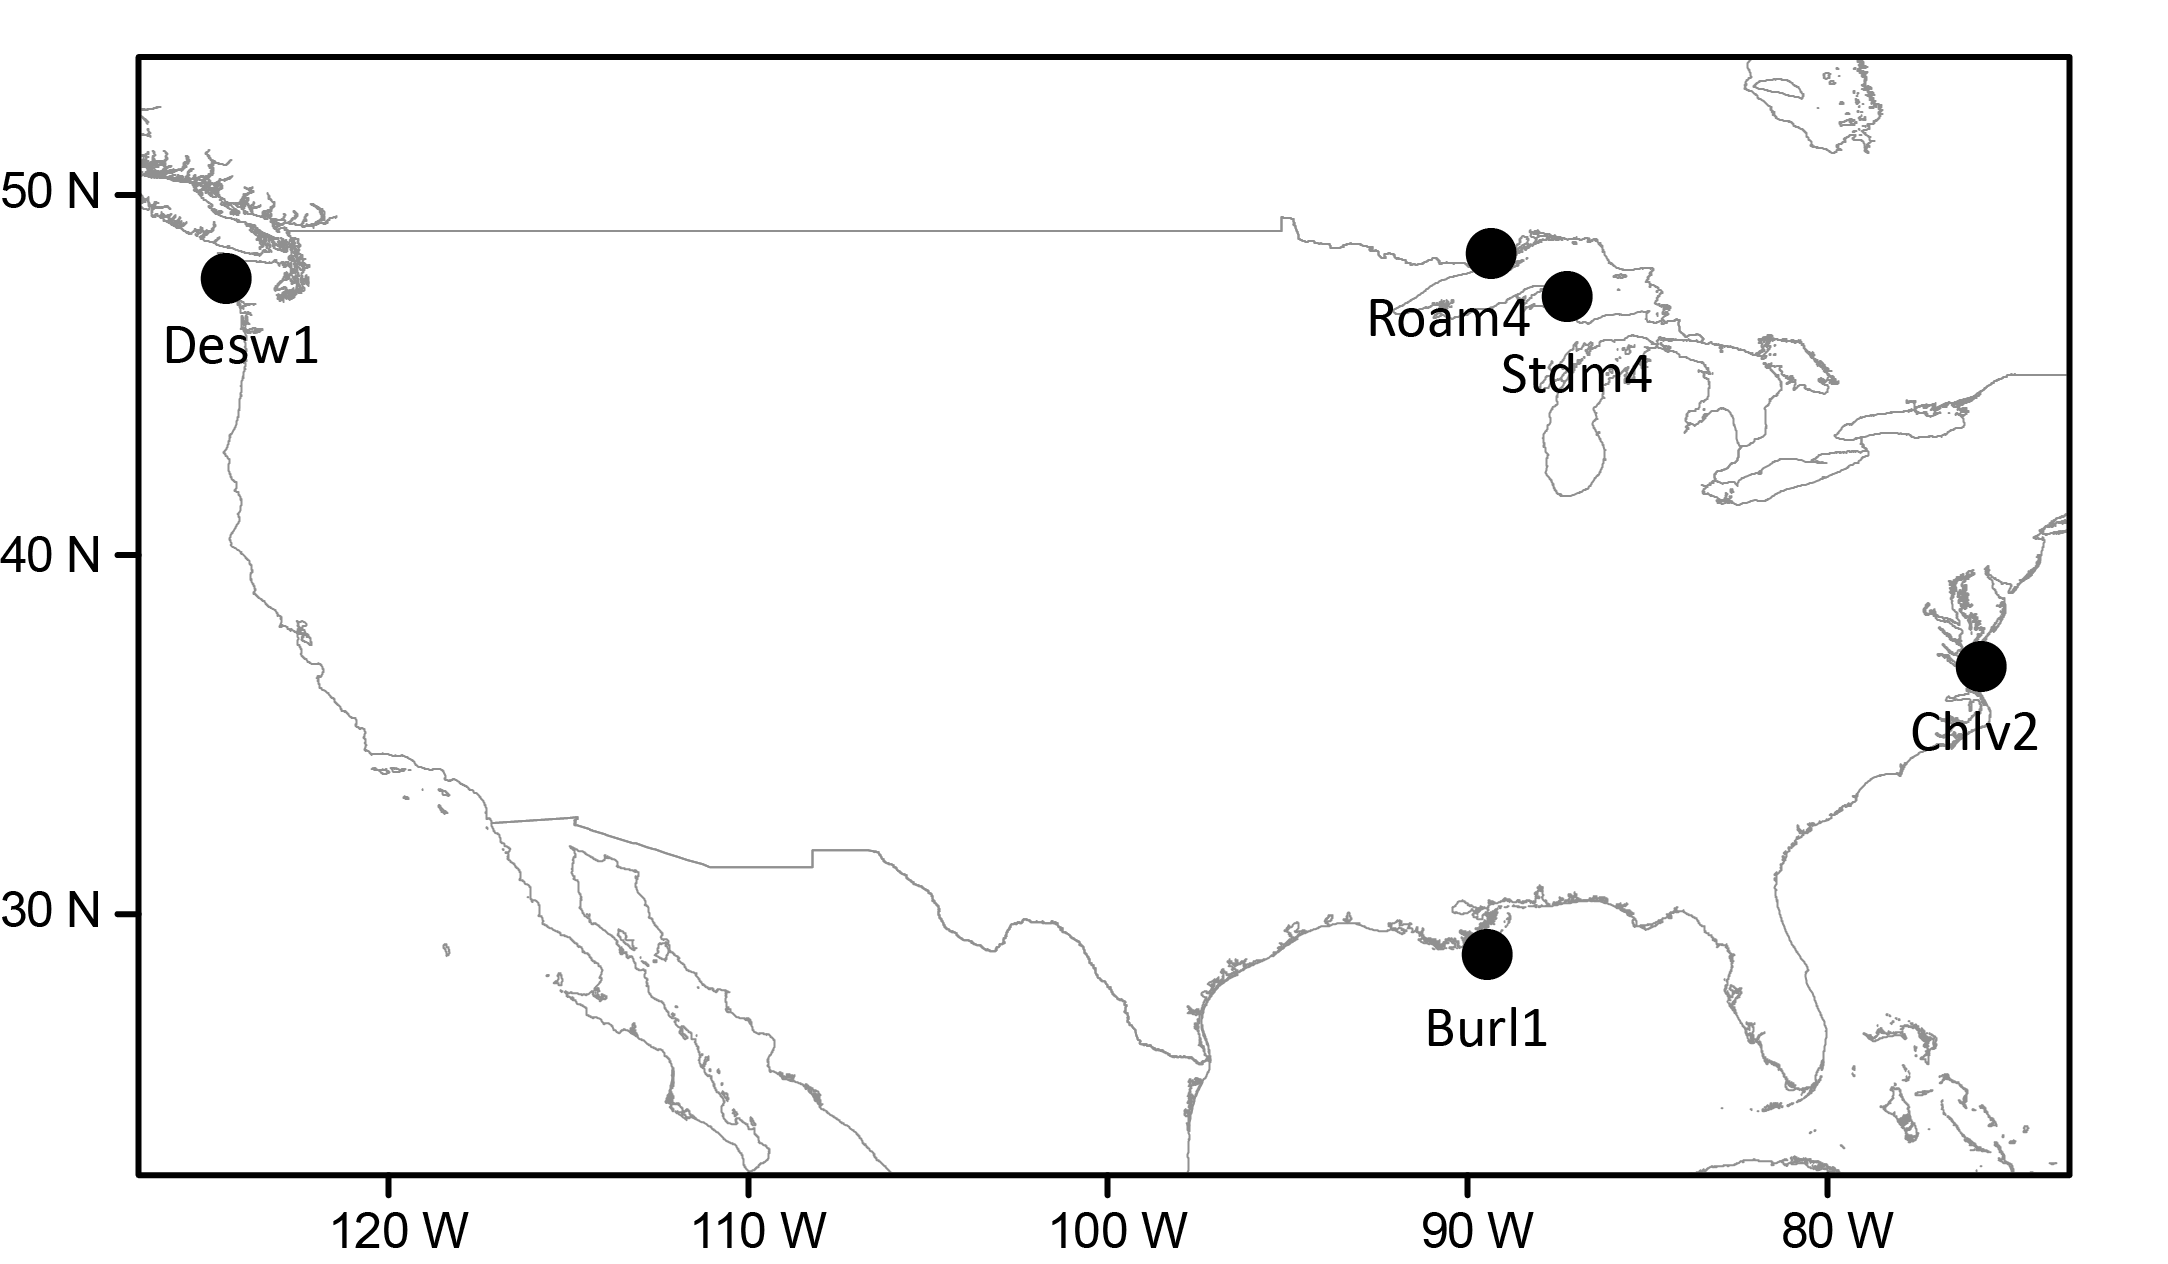
\includegraphics[width=0.75\textwidth]{北美观测塔分布}
    \bicaption{北美观测塔分布}{Locations of observation tower in North America}
    \label{fig:talltower}
\end{figure}

\begin{table}[!htbp]
    \bicaption{观测塔与附近地面站点信息}{Description of observation towers and the surface observation stations close to them}
    \label{tab:stationinfo}
    \centering
    \footnotesize% fontsize
    \setlength{\tabcolsep}{3 pt}% column separation
    \renewcommand{\arraystretch}{1.0}%row space 
    \begin{tabular}{lccccccc}
        \hline
        观测塔名称 & 观测塔经度 & 观测塔纬度 & 风速观测高度 & 距离最近地面 & 站点经度 & 站点纬度 & 风速观测高度 \\
        & & & (地面以上 m)& 站点号 & & &(地面以上 m)\\
        %\cline{2-9}% partial hline from column i to column j
        \hline
        Burl1 & -89.43 & 28.90 & 38 & 994010 & -89.43 & 28.91 & 10 \\
        Chlv2 & -75.71 & 36.91 & 43 & 723075 & -76.03 & 36.82 & 10 \\
        Desw1 & -124.49 & 47.68 & 31 & 727970 & -124.55 & 47.94 & 10 \\
        Roam4 & -89.31 & 47.87 & 47 & 717490 & -89.33 & 48.37 & 10 \\
        Stdm4 & -87.23 & 47.18 & 35 & 727440 & -88.49 & 47.17 & 10 \\ 
        \hline
    \end{tabular}
\end{table}

\begin{figure}[!htbp]
    \centering
    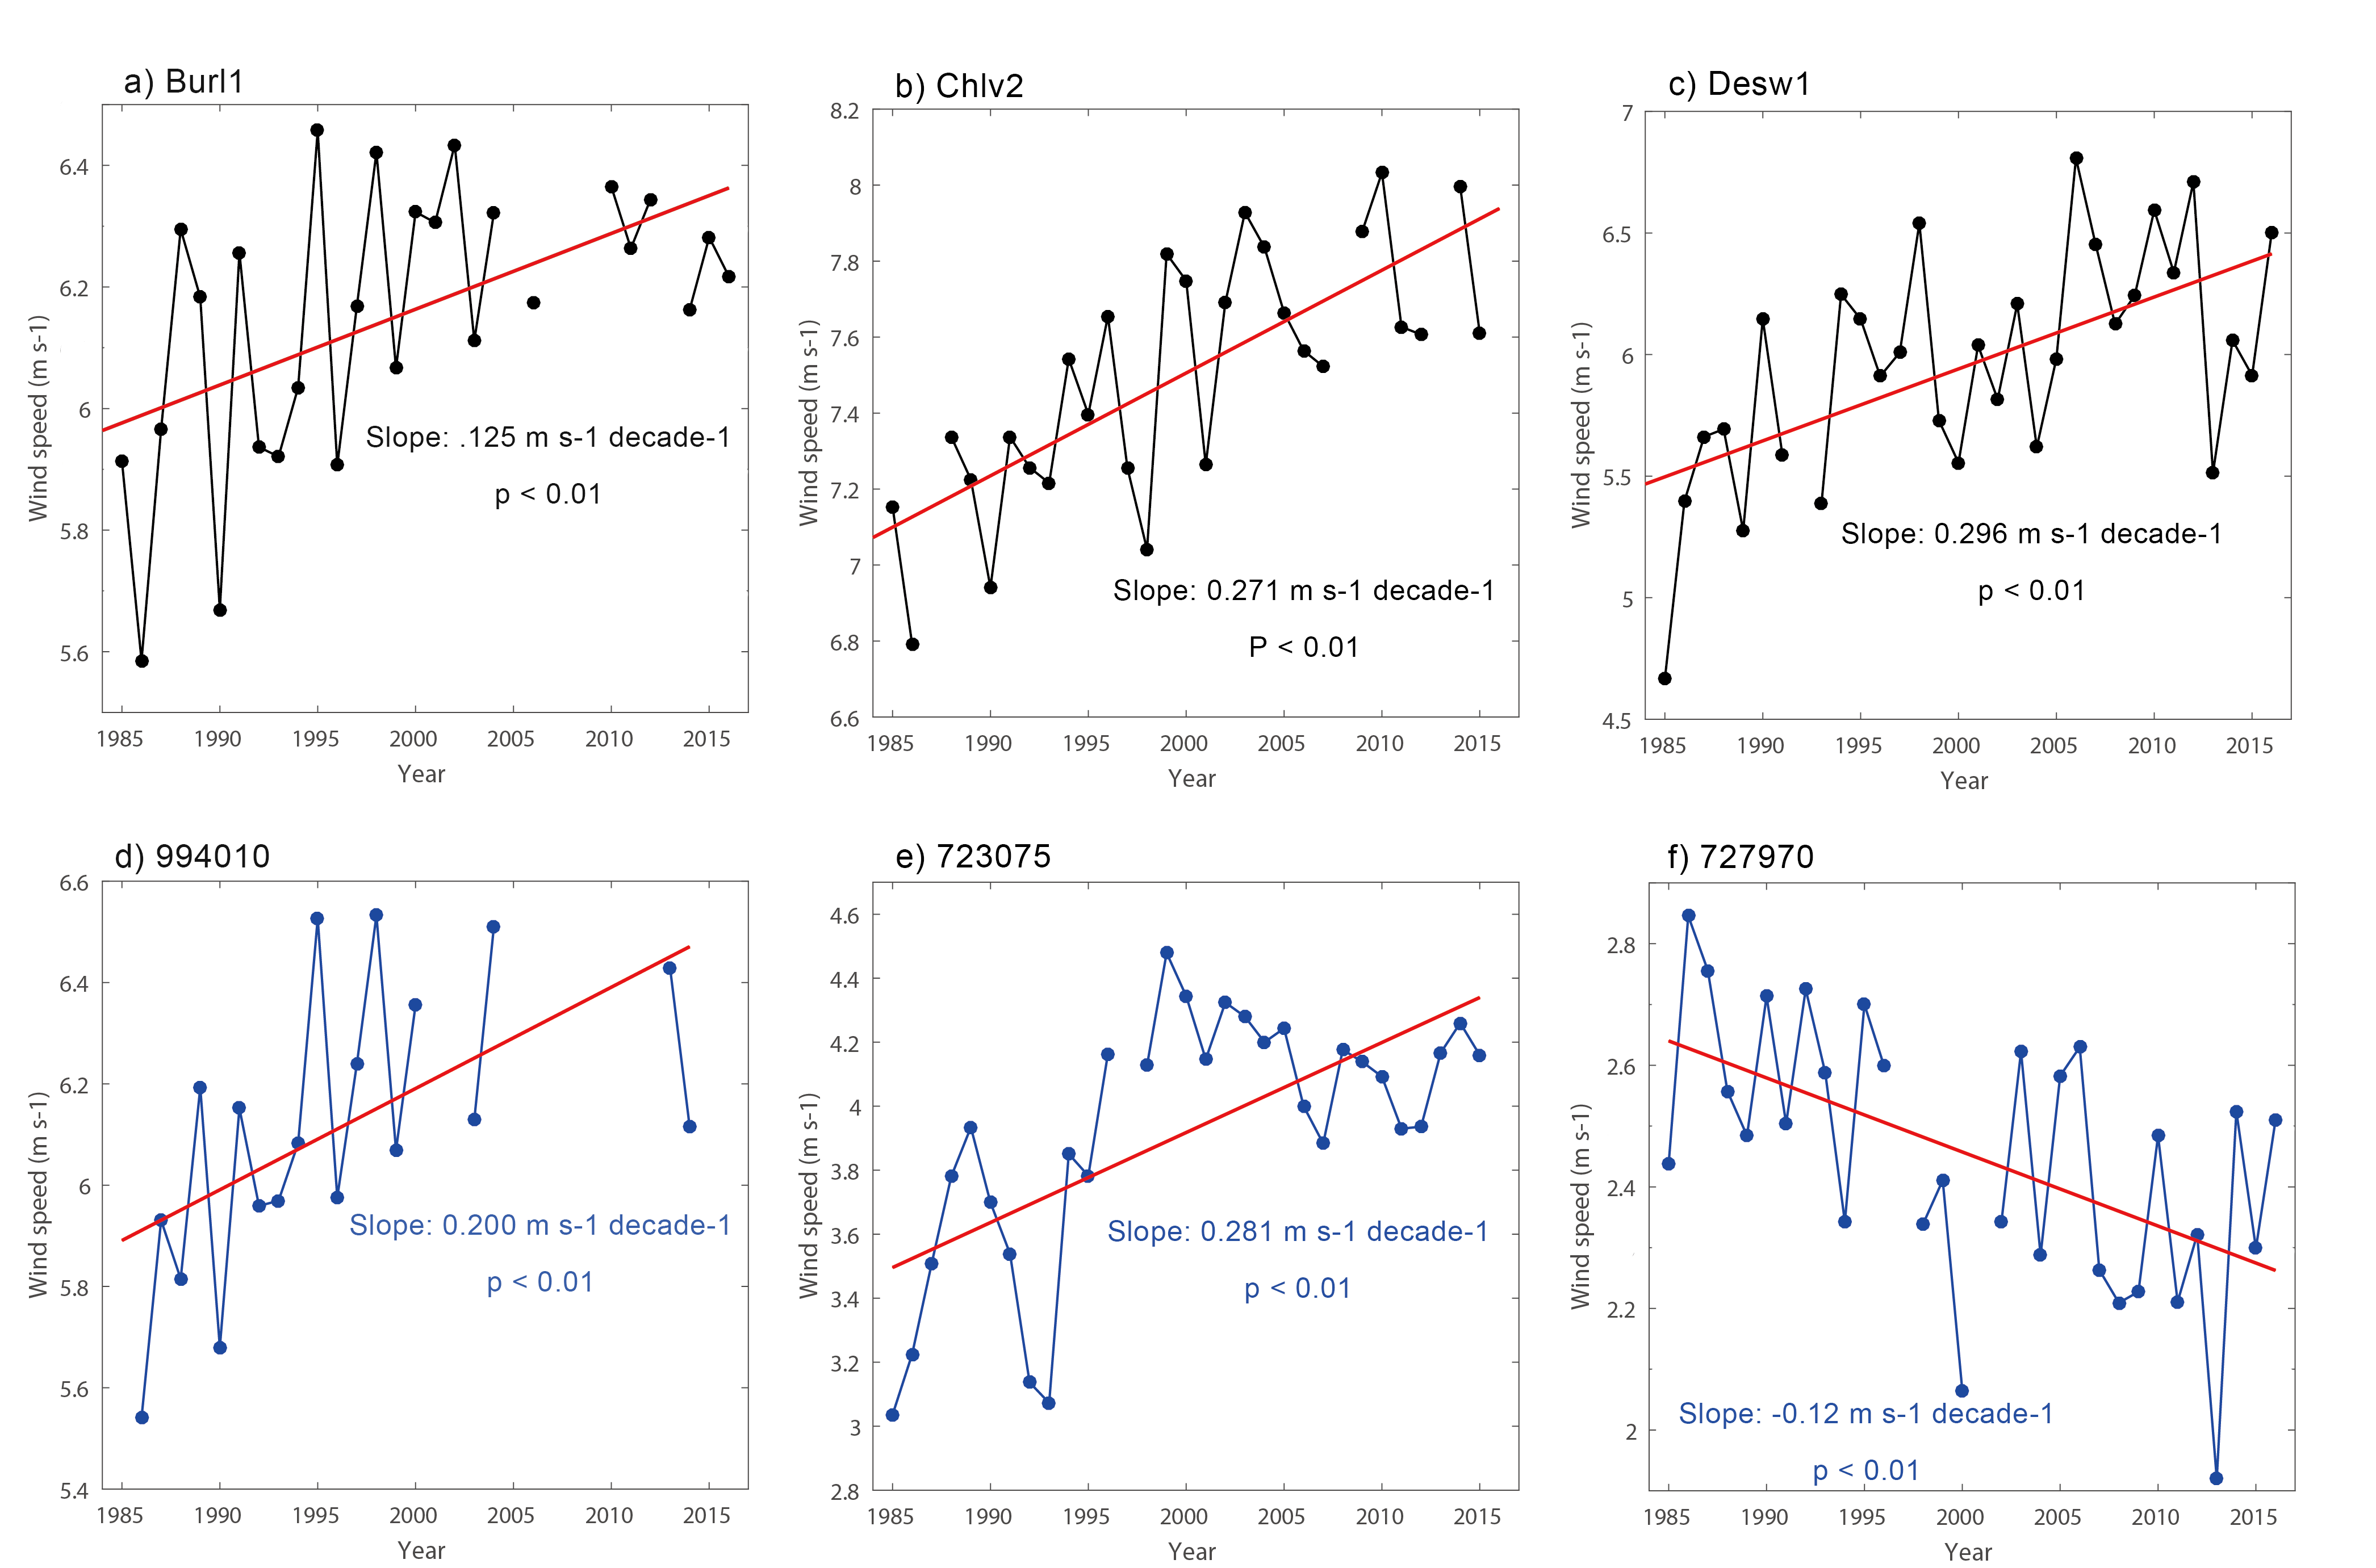
\includegraphics[width=1\textwidth]{北美观测塔风速趋势1}
    \bicaption{北美观测塔风速趋势(第一部分)。d)994010、e)723075、f)727970分别为距离观测塔a)Burl1、b)Chlv2、c)Desw1最近的地面观测站点。}{Wind speed trends of observation tower in North America (part 1). d)994010, e)723075, f)727970 are surface observation stations closest to a)Burl1, b)Chlv2, c)Desw1, respectively.}
    \label{fig:talltowerwindtrend1}
\end{figure}

\begin{figure}[!t]
    \centering
    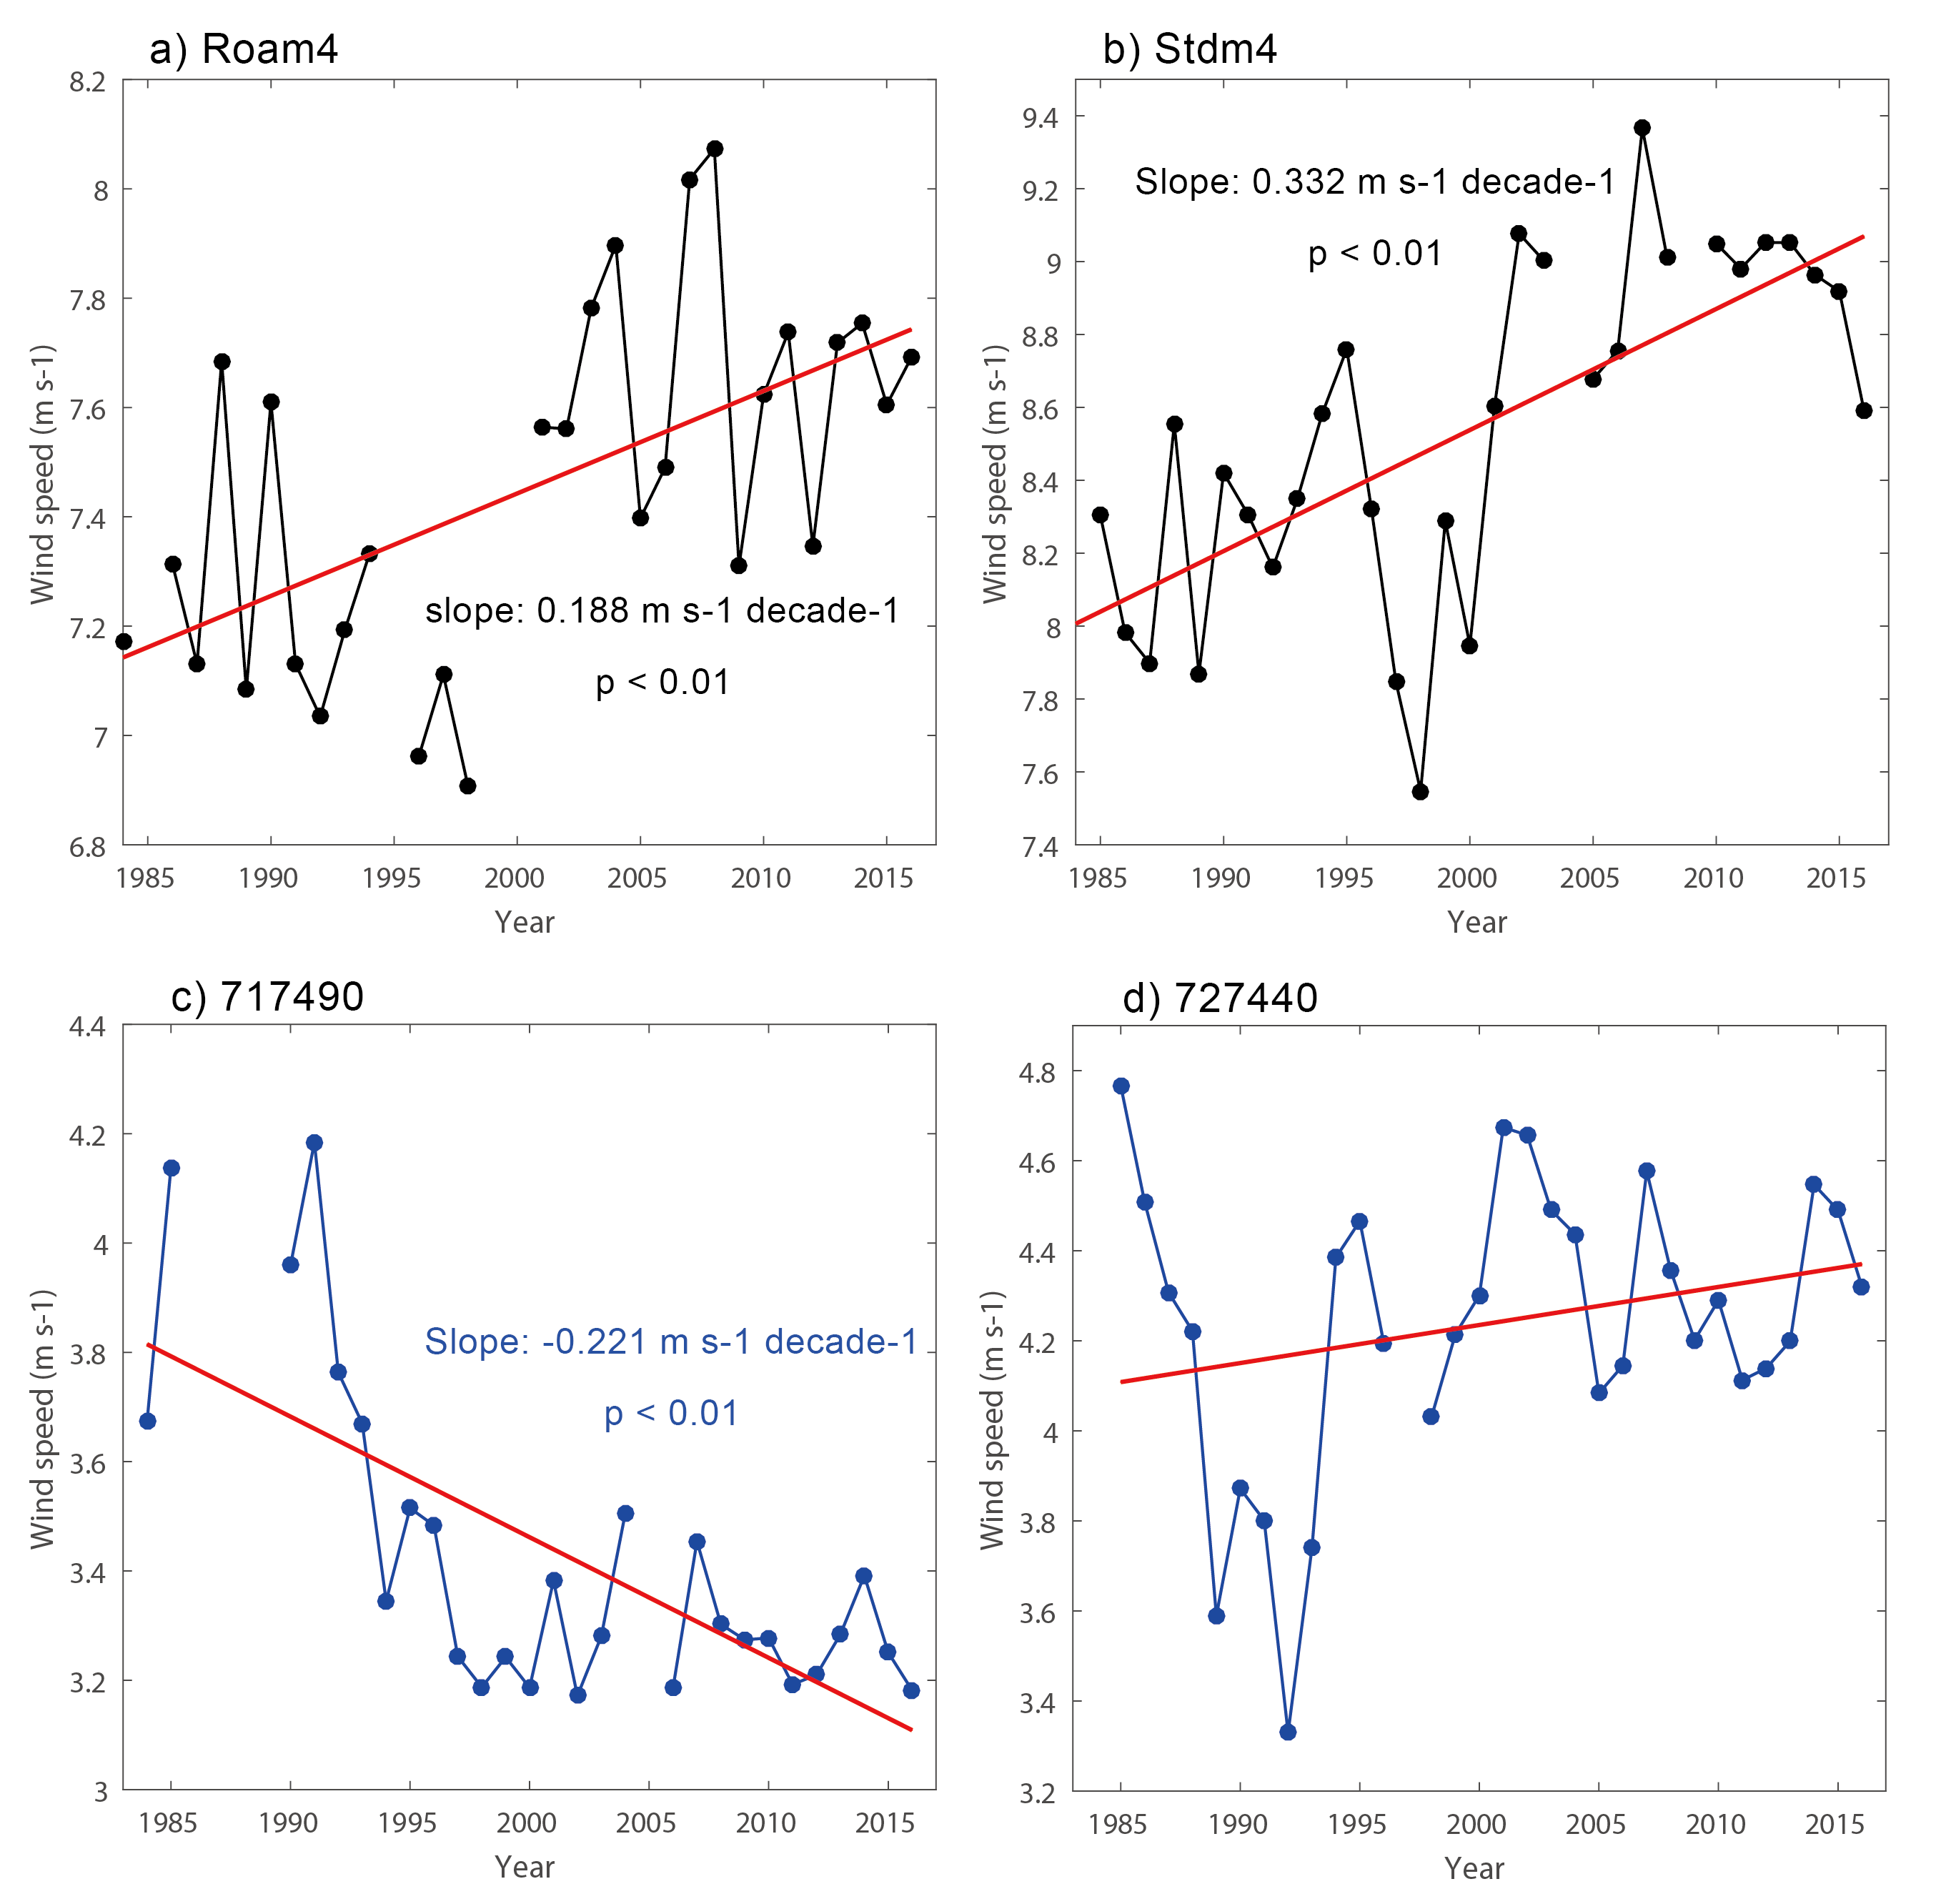
\includegraphics[width=0.65\textwidth]{北美观测塔风速趋势2}
    \bicaption{北美观测塔风速趋势(第二部分)。c)717490、d)727440分别为距离观测塔a)Roam4、b)Stdm4最近的地面观测站点。}{Wind speed trends of observation tower in North America (part 2). c)717490、d)727440 are surface observation stations closest to a)Roam4、b)Stdm4, respectively.}
    \label{fig:talltowerwindtrend2}
\end{figure}

\subsection{对流层风速年代际变化}

全球平均来看,地表风速在2007年前迅速下降,气候趋于平稳;850 hPa风速先上升(1990年前),后下降(1990-2000),再上升(2000年后)三个阶段;700 hPa在2005年前与850 hPa变化类似,2005年后趋于平稳;500 hPa风速在1995年前快速上升,气候缓慢下降;200 hPa风速1990年前缓慢下降,1990-2000快速上升,其后又缓慢下降(图 \ref{fig:globaltroposhereevolution})。在北美洲,地表风速经历了1987年前平稳时期,1987-2000缓慢下降时期,2000-2010快速下降时期和2010年后平稳时期;850和700 hPa,风速表现为1995年前快速上升时期,1995-2005缓慢上升时期和2005年后缓慢下降时期;500 hPa风速在1995年前快速上升,1995-2003缓慢下降,2003-2013又快速上升,其后在此出现下降;200 hPa风速在1988年前缓慢下降,1988-1995快速上升,1995-2005趋于平稳,2005年后再次快速上升(图 \ref{fig:NAtroposhereevolution})。在欧洲,地表风速1990年前快速下降,1990-2000中速下降,2000年后慢速下降;850和700 hPa年代际变化较为类似,均在1985年前无明显变化,1985-1993上升,1993-2003下降,不同之处在于850 hPa在2003年后又开始缓慢上升,而700 hPa趋于平稳;500和200 hPa,风速均经历了1990年前平稳时期,1990-2000年上升时期,2000-2010年下降时期和2010年后再次缓慢上升时期(图 \ref{fig:EUtroposhereevolution})。在亚洲低纬度地区,地表风速在1987年前快速下降,1987-1995年微弱上升,之后又快速下降;850 hPa在1990年前微弱上升,之后快速下降直到2000年,其后2000-2010再次缓慢上升,后又下降;700 hPa年代际变化不明显;500 hPa风速在1990年前缓慢上升,1990-2000缓慢下降,2000-2010快速上升,其后缓慢下降;200 hPa风速以2000年为界,前期风速上升,后期风速下降(图 \ref{fig:ASlowtroposhereevolution})。在亚洲中纬度地区,地表风速在1990年前快速下降,1990-1997年趋于平稳,1997-2007再次快速下降,2007年后再次趋于平稳;850 hPa和700 hPa风速变化都以1990和2000为界分为三个时期,850 hPa风速在这三个时期表现分别为平稳、下降和上升,而700 hPa表现为缓慢下降,快速下降和上升;500 hPa风速没有表现出明显年代际变化;200 hPa风速仅在1993-2003有一段上升时期,之前和之后风速均较为平稳(图 \ref{fig:ASmidtroposhereevolution})。

\begin{figure}[!htbp]
    \centering
    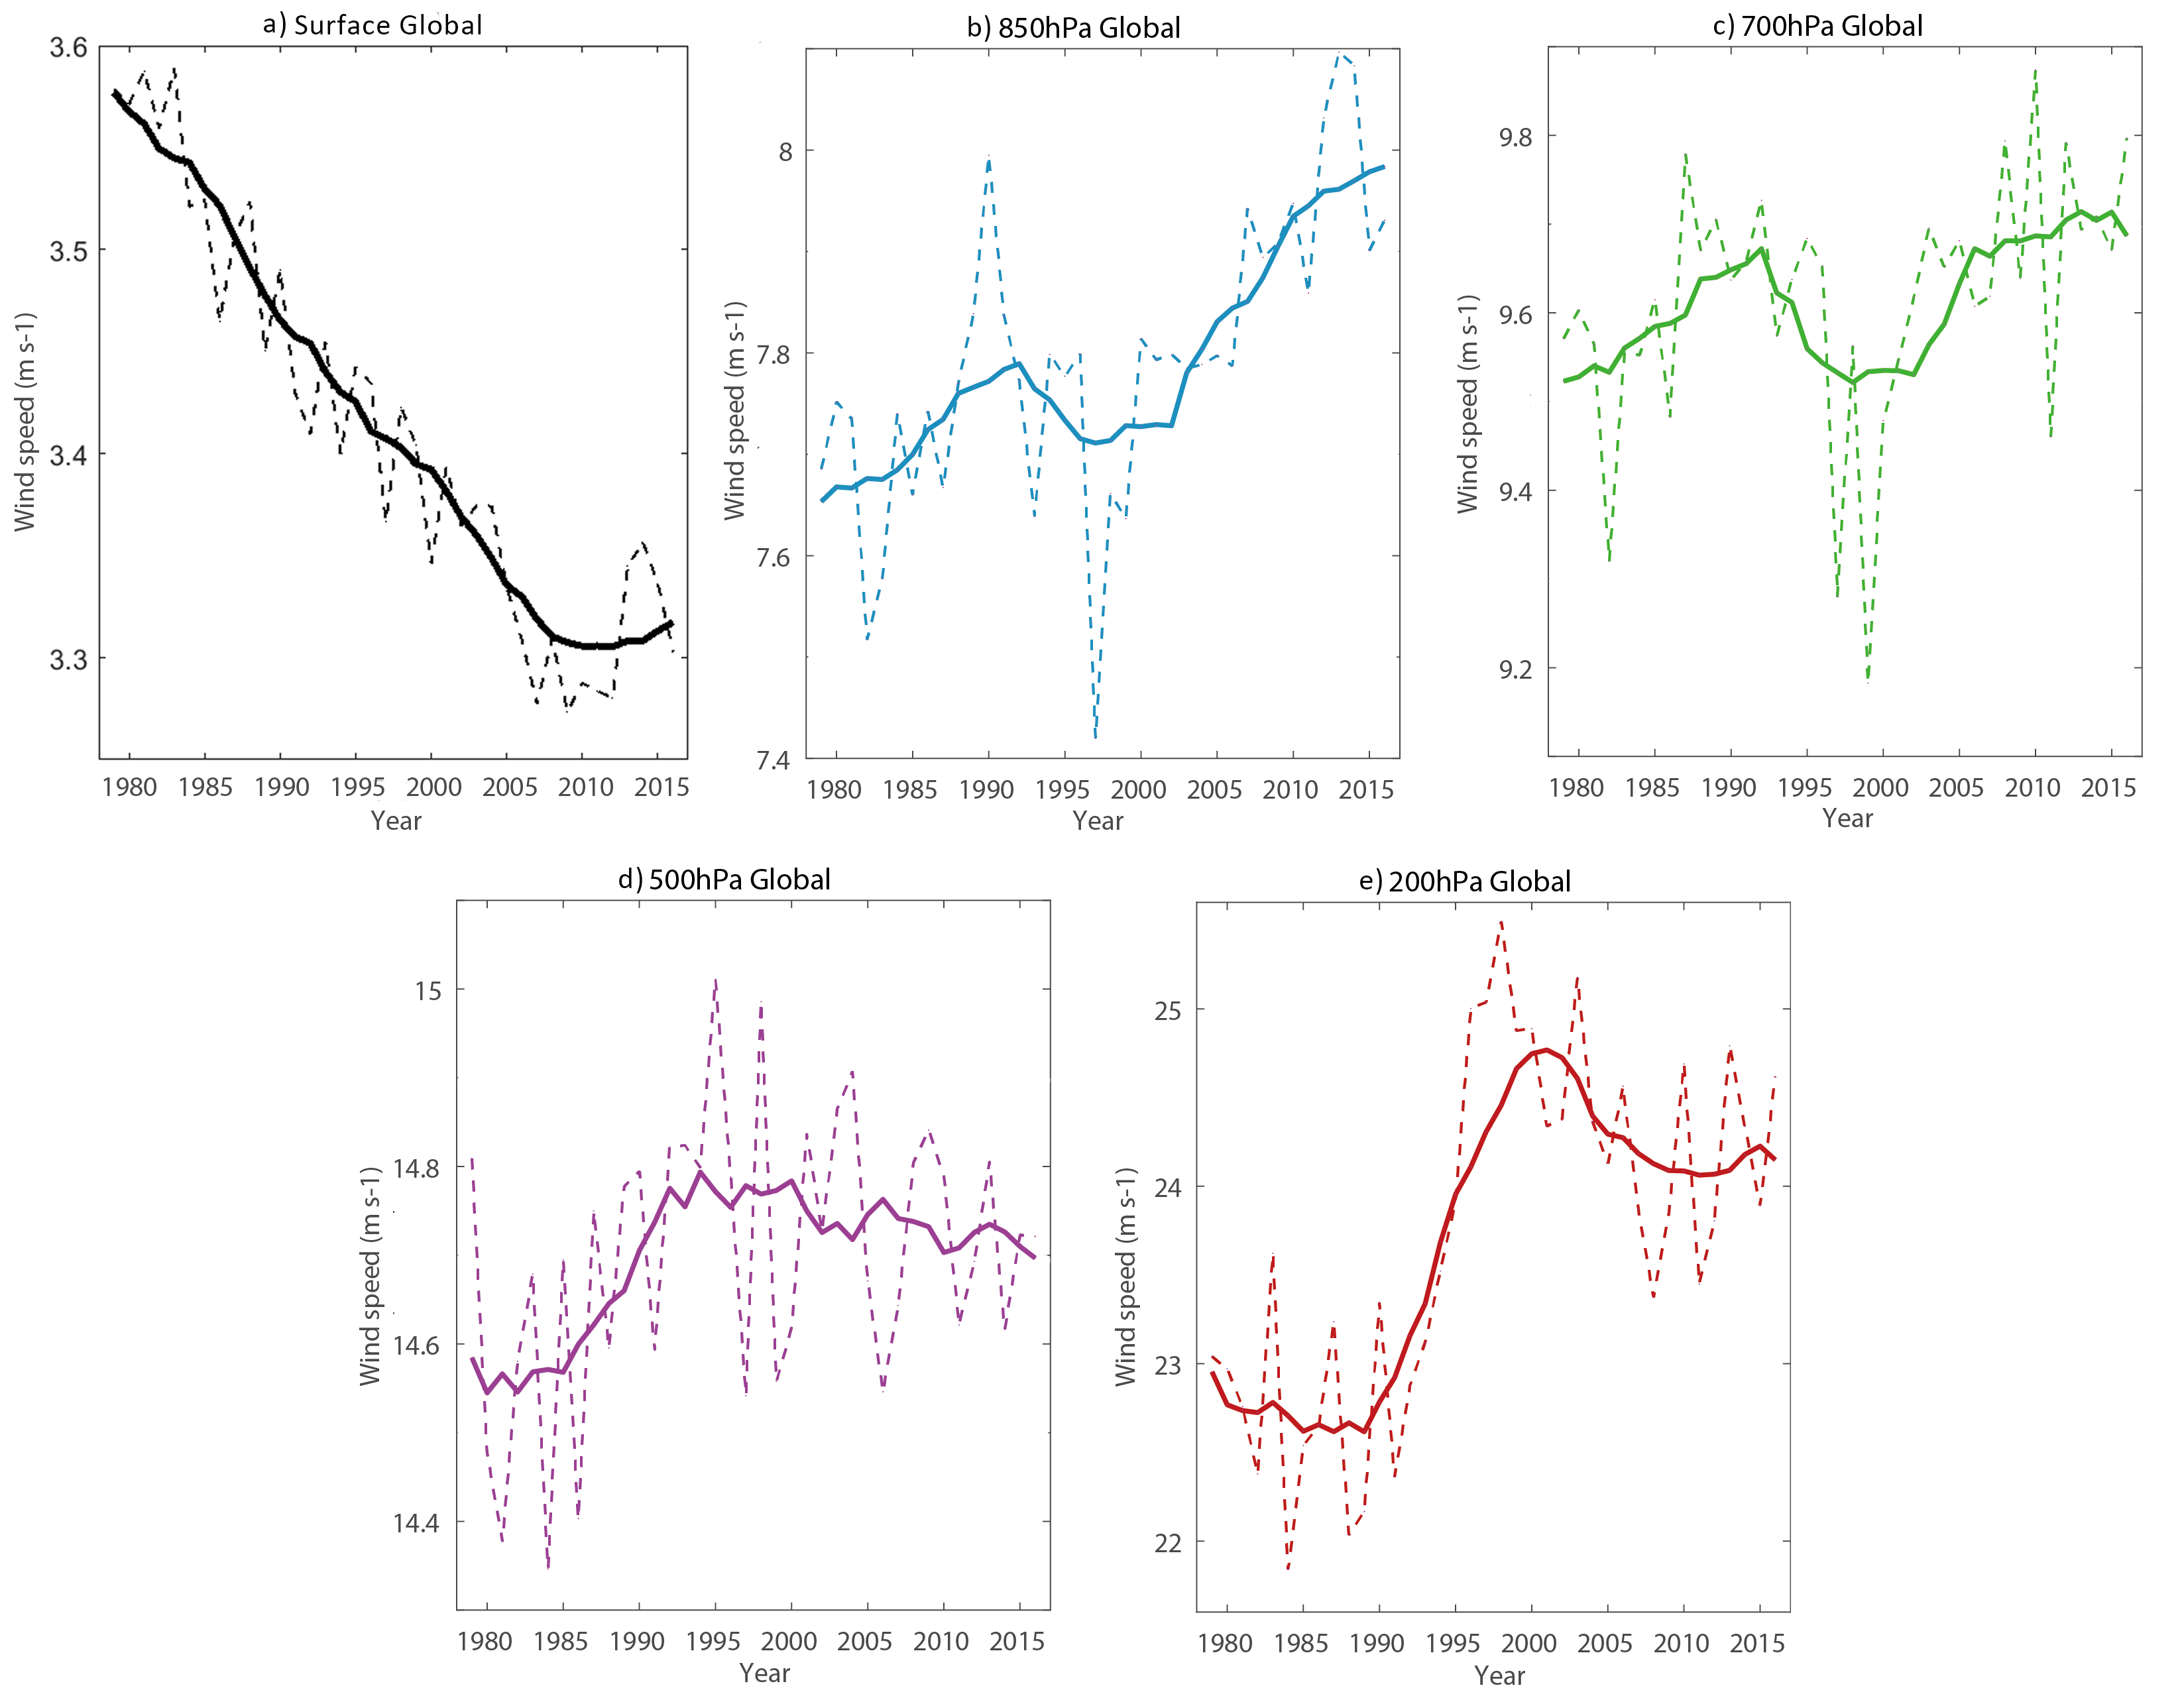
\includegraphics[width=0.85\textwidth]{全球对流层中位数风速演变}
    \bicaption{全球对流层中位数风速演变($m ~ s^{-1}$)。a)地面,b)850 hPa,c)700 hPa,d)500 hPa,e)200 hPa。虚线为各年对应值,实线为虚线9点平滑的结果。}{Global median troposhere wind speed evolution (in $m ~ s^{-1}$). a)Surface, b)850 hPa, c)700 hPa, d)500 hPa, e)200 hPa. Dash line denotes values for every year, solid line is 9-point moving mean of dash line.}
    \label{fig:globaltroposhereevolution}
\end{figure}

\begin{figure}[!t]
    \centering
    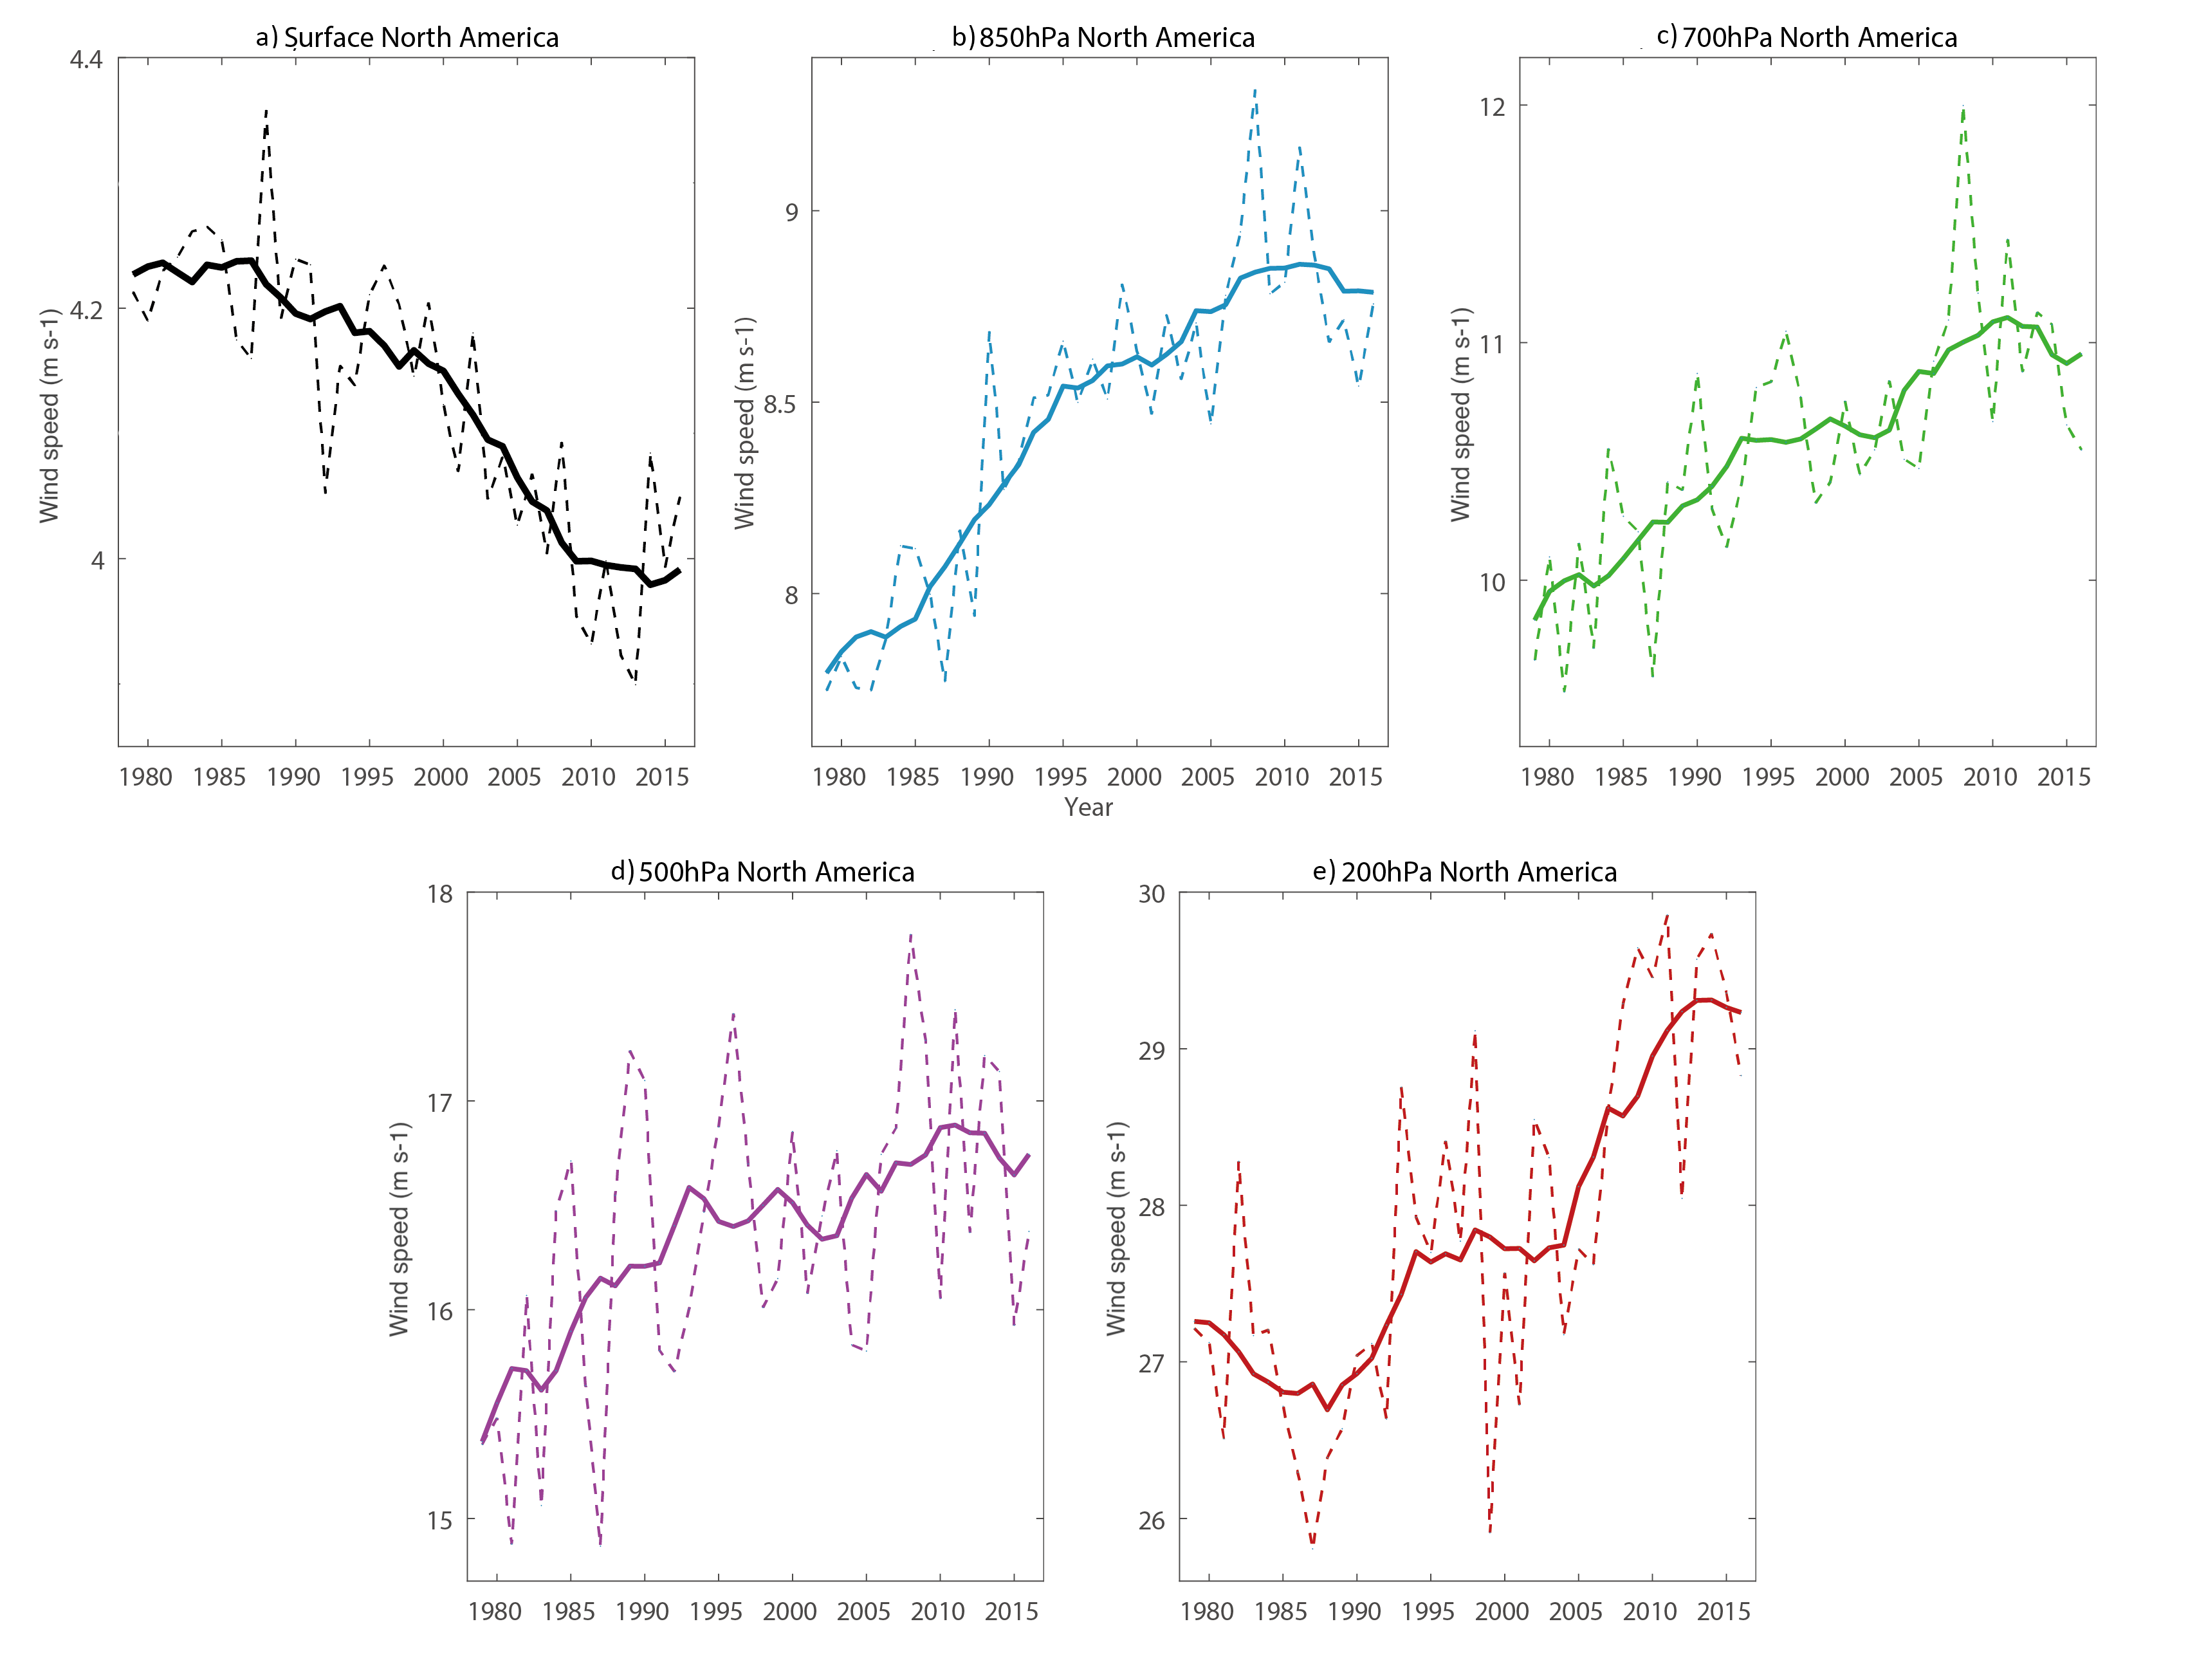
\includegraphics[width=0.85\textwidth]{北美对流层中位数风速演变}
    \bicaption{北美洲对流层中位数风速演变($m ~ s^{-1}$)。与图 \ref{fig:globaltroposhereevolution}类似。}{North American median troposhere wind speed evolution (in $m ~ s^{-1}$). Same as \ref{fig:globaltroposhereevolution}, but for North America.}
    \label{fig:NAtroposhereevolution}
\end{figure}

\begin{figure}[!b]
    \centering
    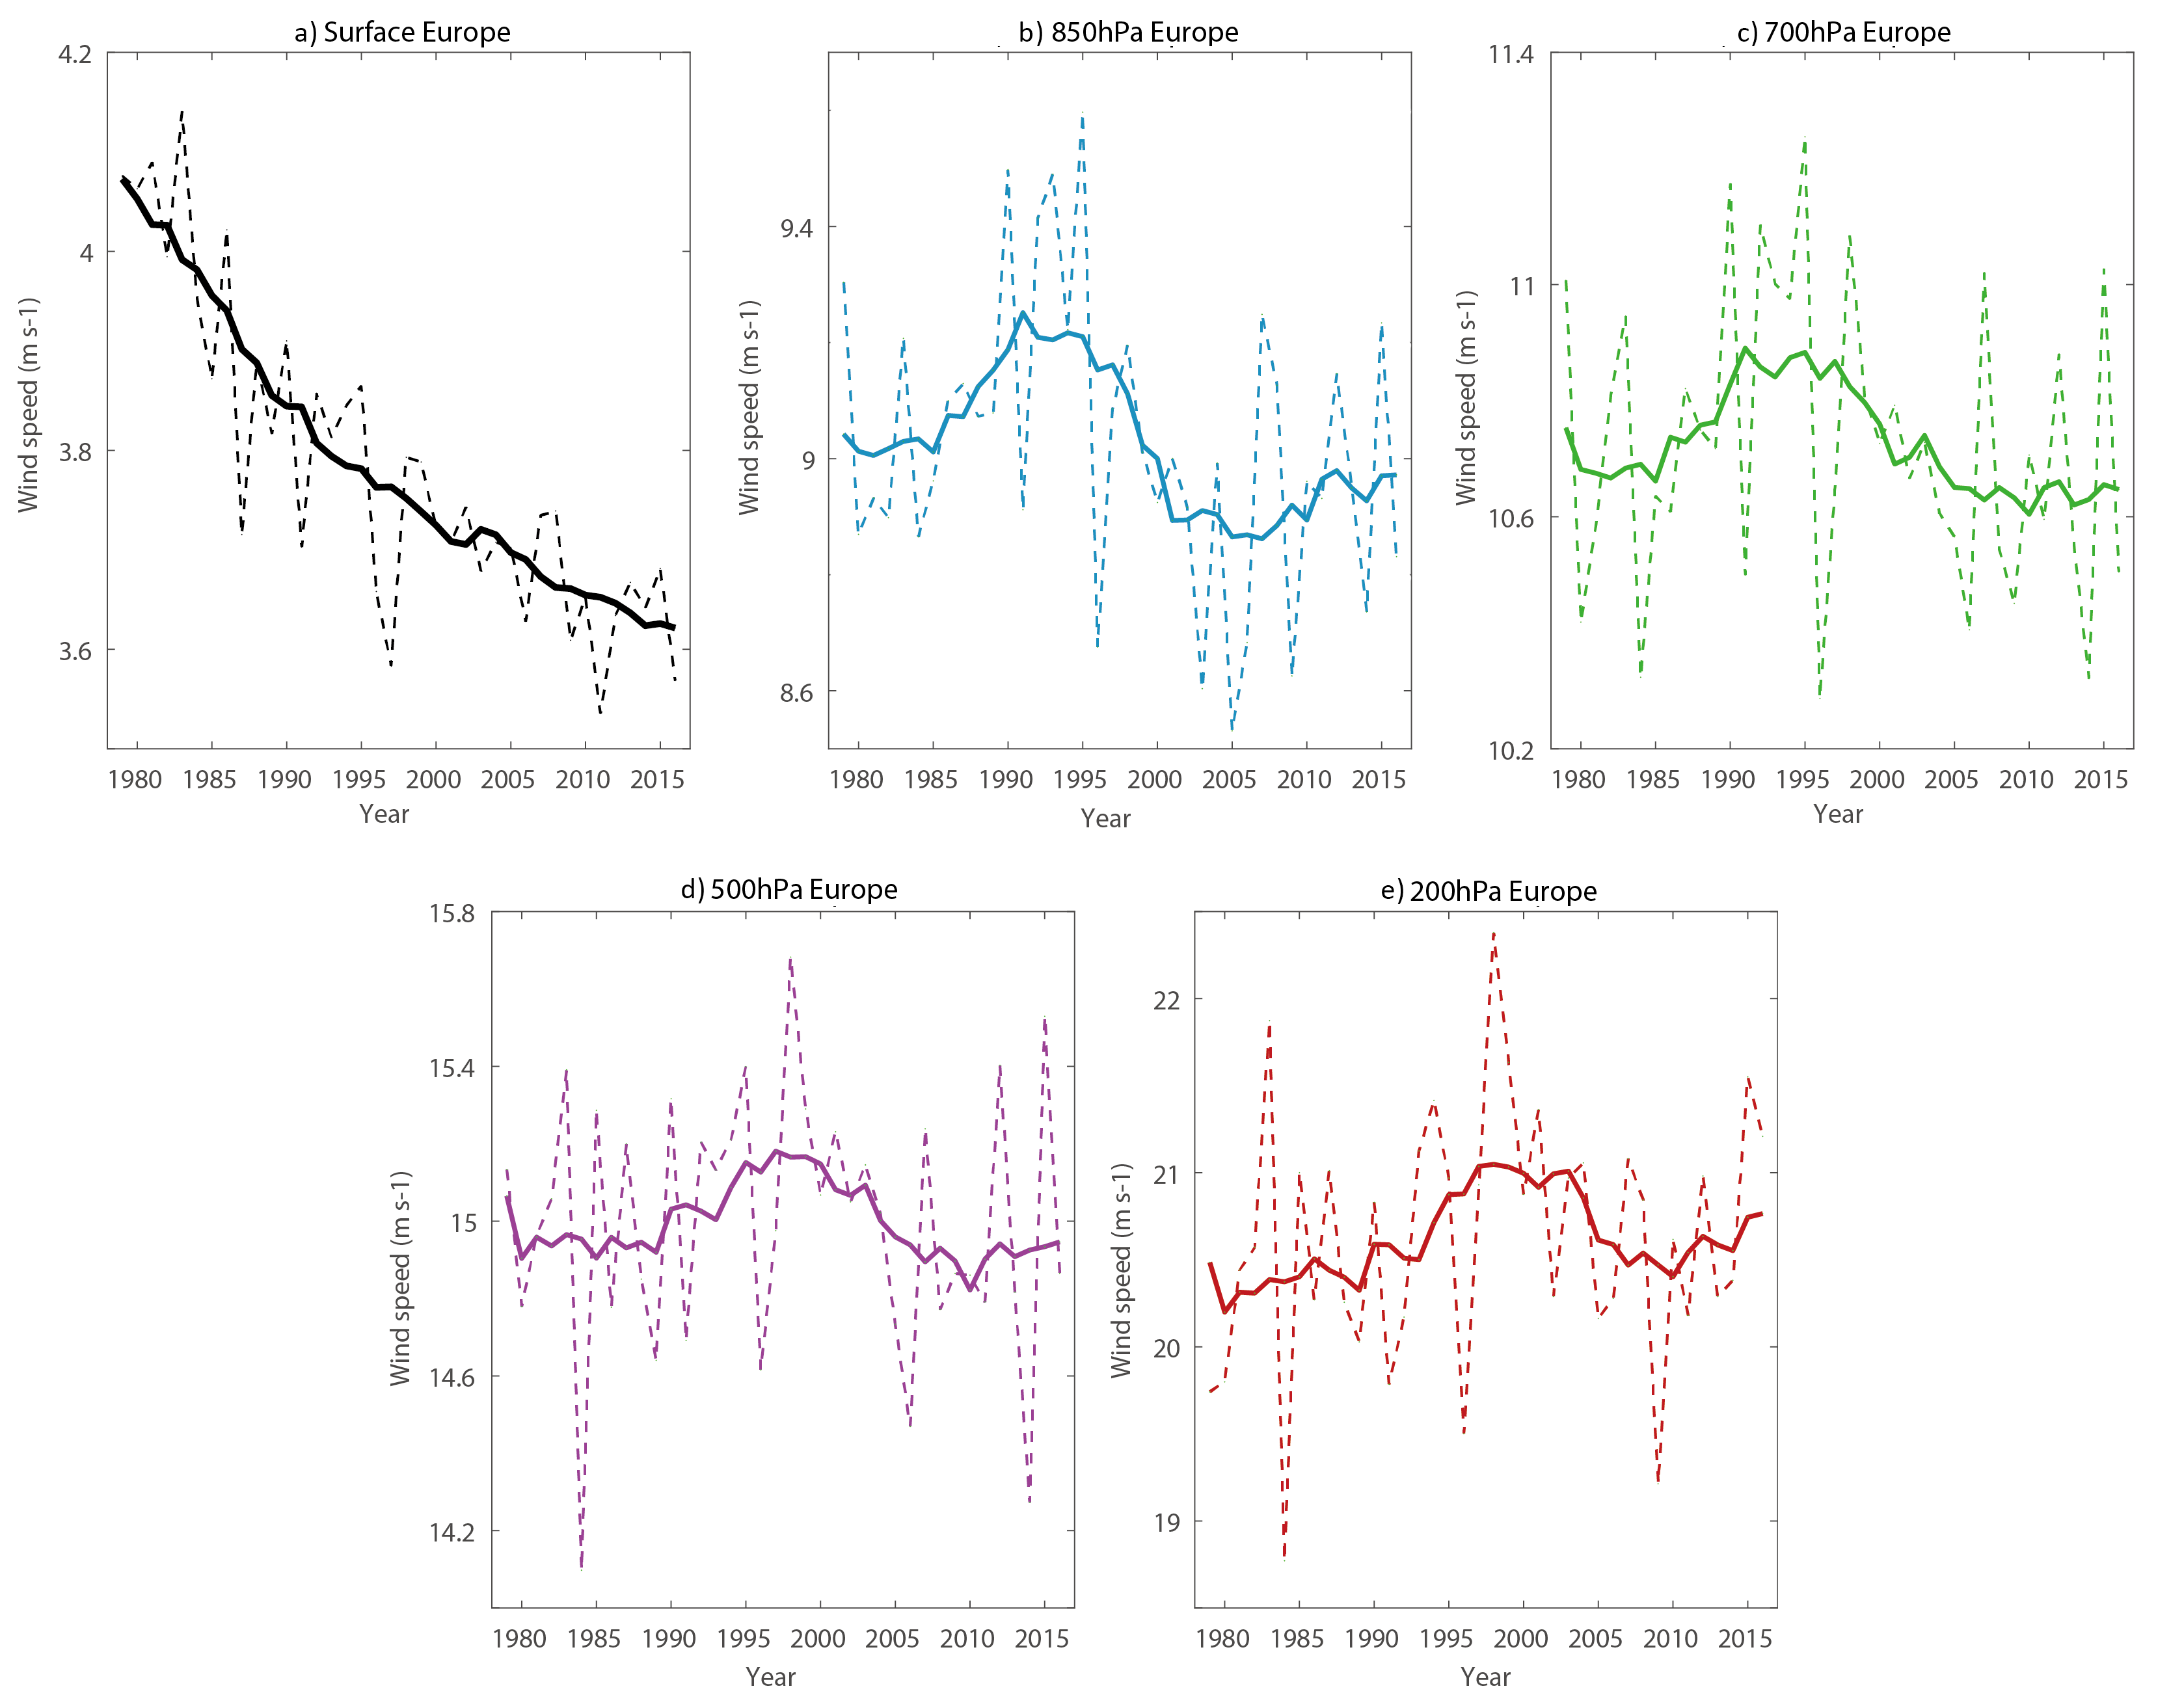
\includegraphics[width=0.85\textwidth]{欧洲对流层中位数风速演变}
    \bicaption{欧洲对流层中位数风速演变($m ~ s^{-1}$)。与图 \ref{fig:globaltroposhereevolution}类似。}{European median troposhere wind speed evolution (in $m ~ s^{-1}$). Same as \ref{fig:globaltroposhereevolution}, but for Europe.}
    \label{fig:EUtroposhereevolution}
\end{figure}

\begin{figure}[!t]
    \centering
    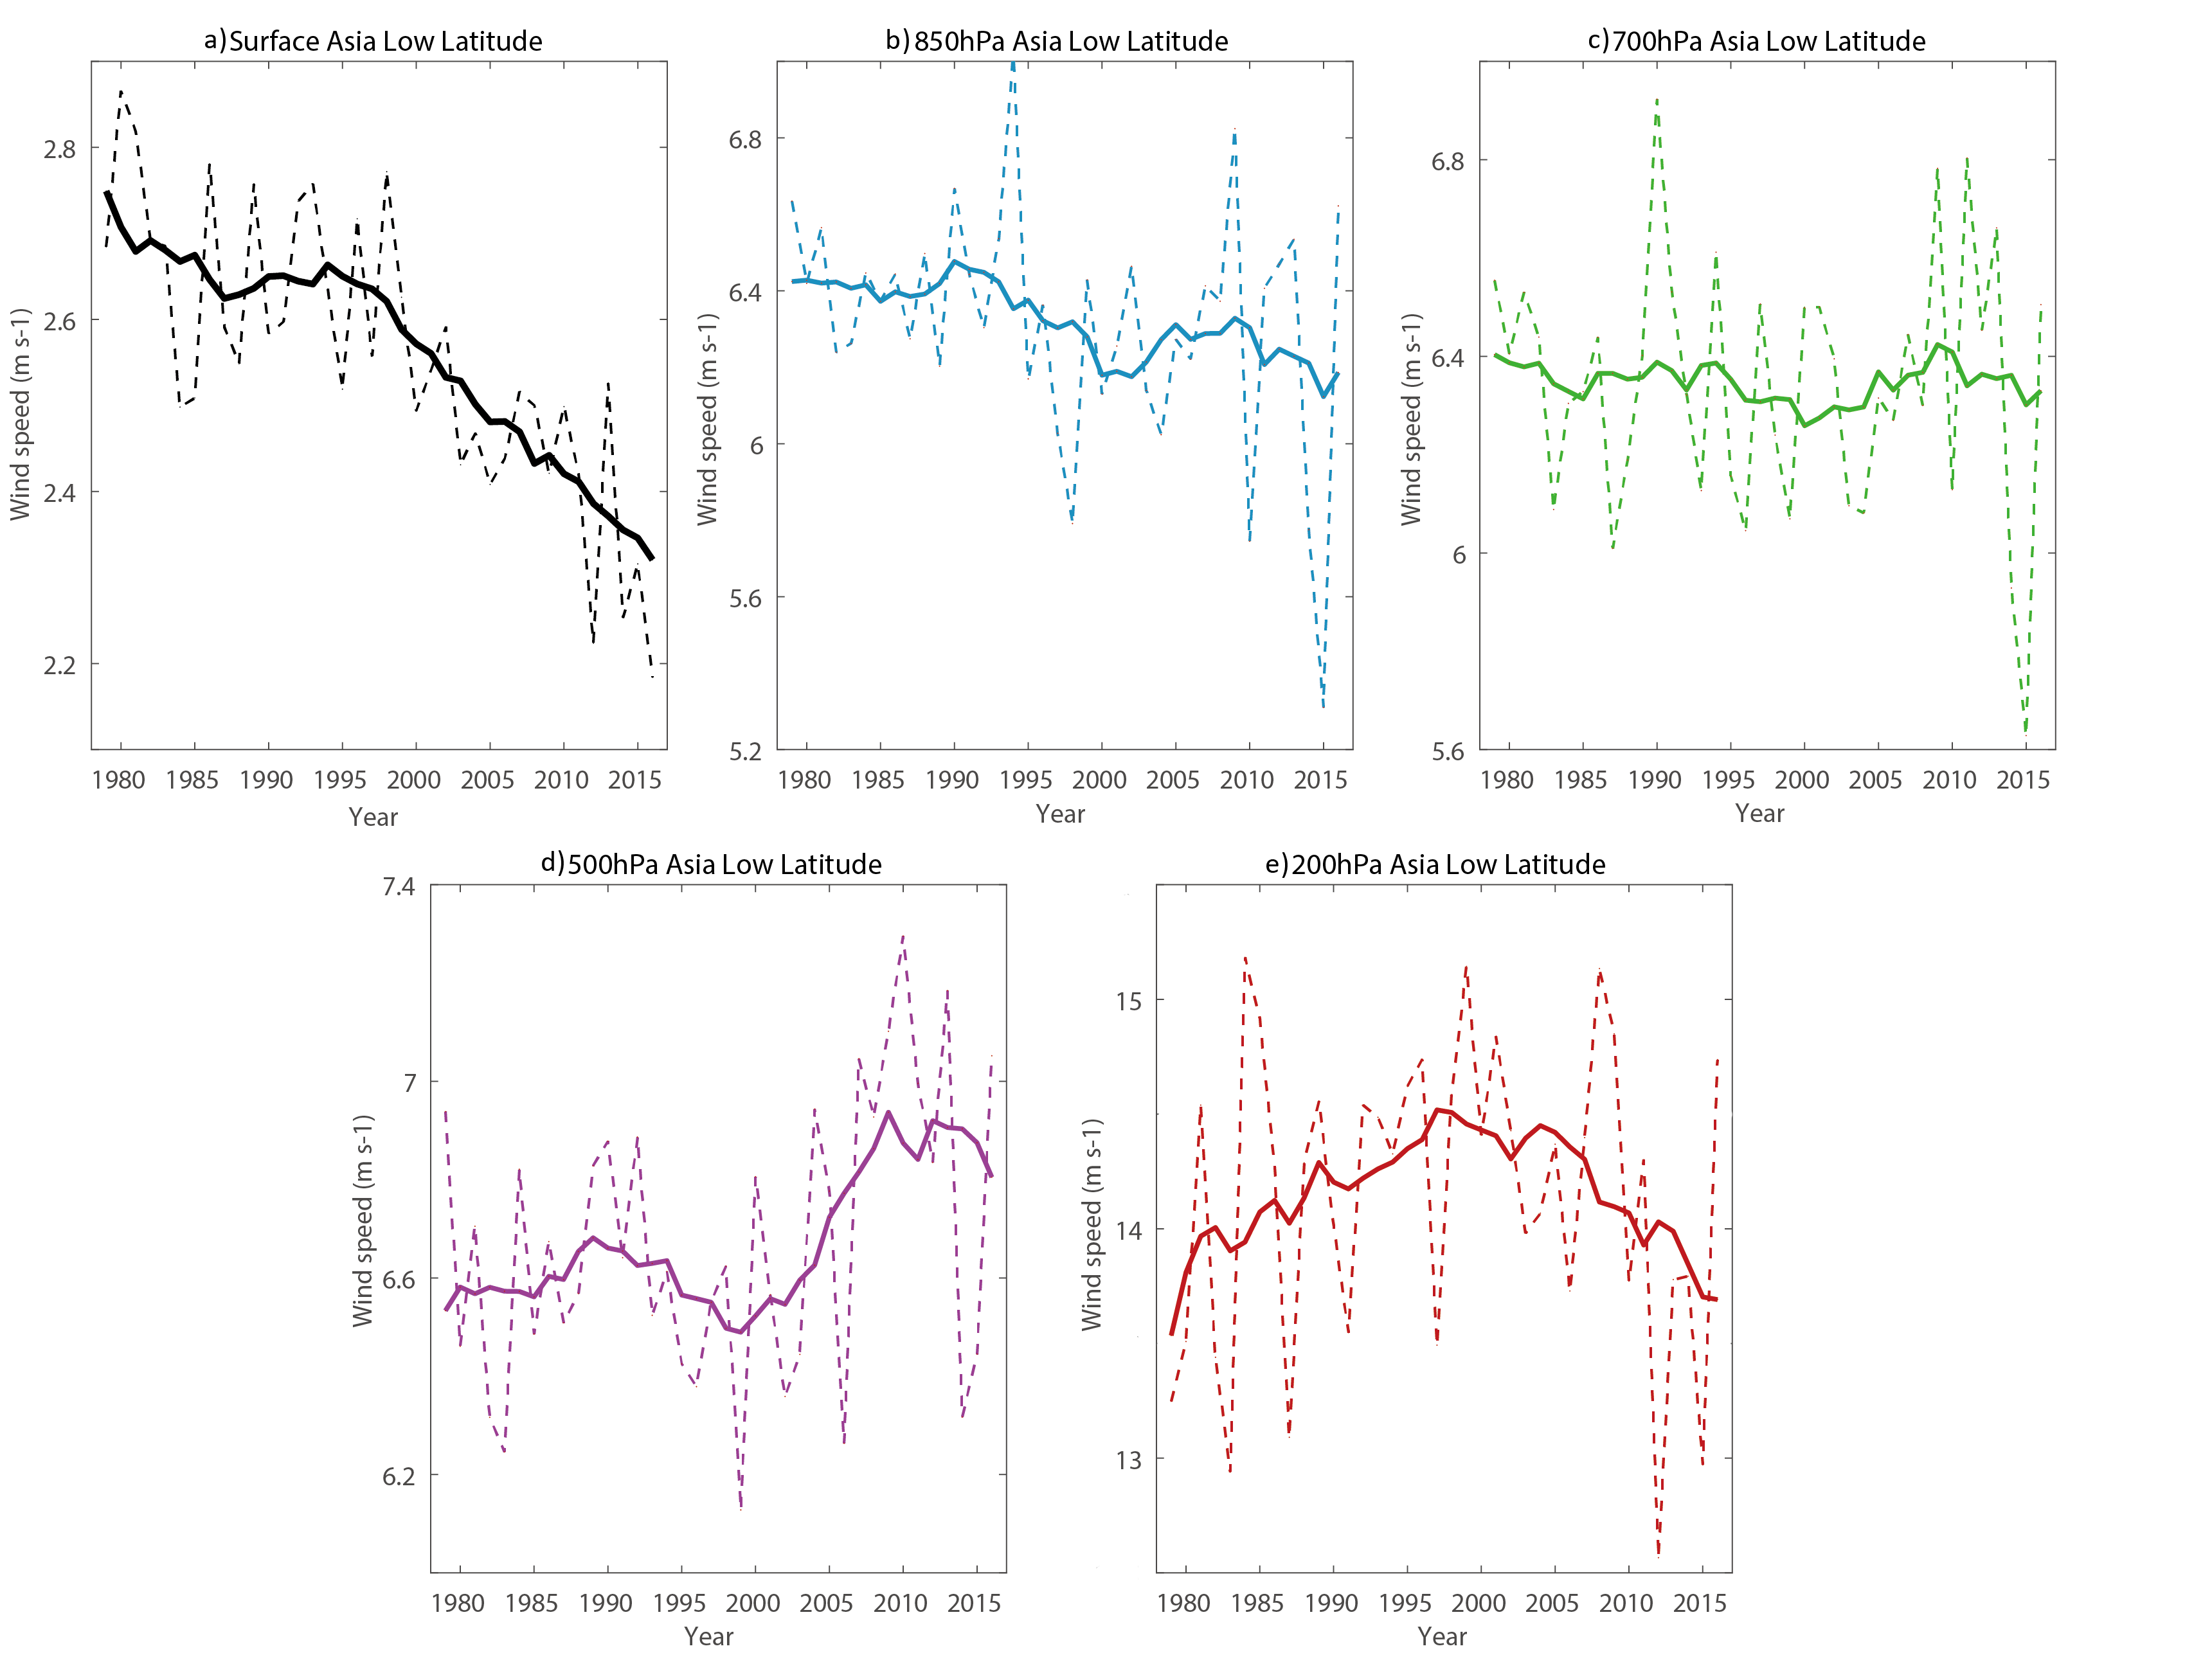
\includegraphics[width=0.85\textwidth]{亚洲低纬度对流层中位数风速演变}
    \bicaption{亚洲低纬度(0 - 20 N)对流层中位数风速演变($m ~ s^{-1}$)。与图 \ref{fig:globaltroposhereevolution}类似。}{Asian low latitude (0 - 20 N) median troposhere wind speed evolution (in $m ~ s^{-1}$). Same as \ref{fig:globaltroposhereevolution}, but for Asia low latitude.}
    \label{fig:ASlowtroposhereevolution}
\end{figure}

\begin{figure}[!b]
    \centering
    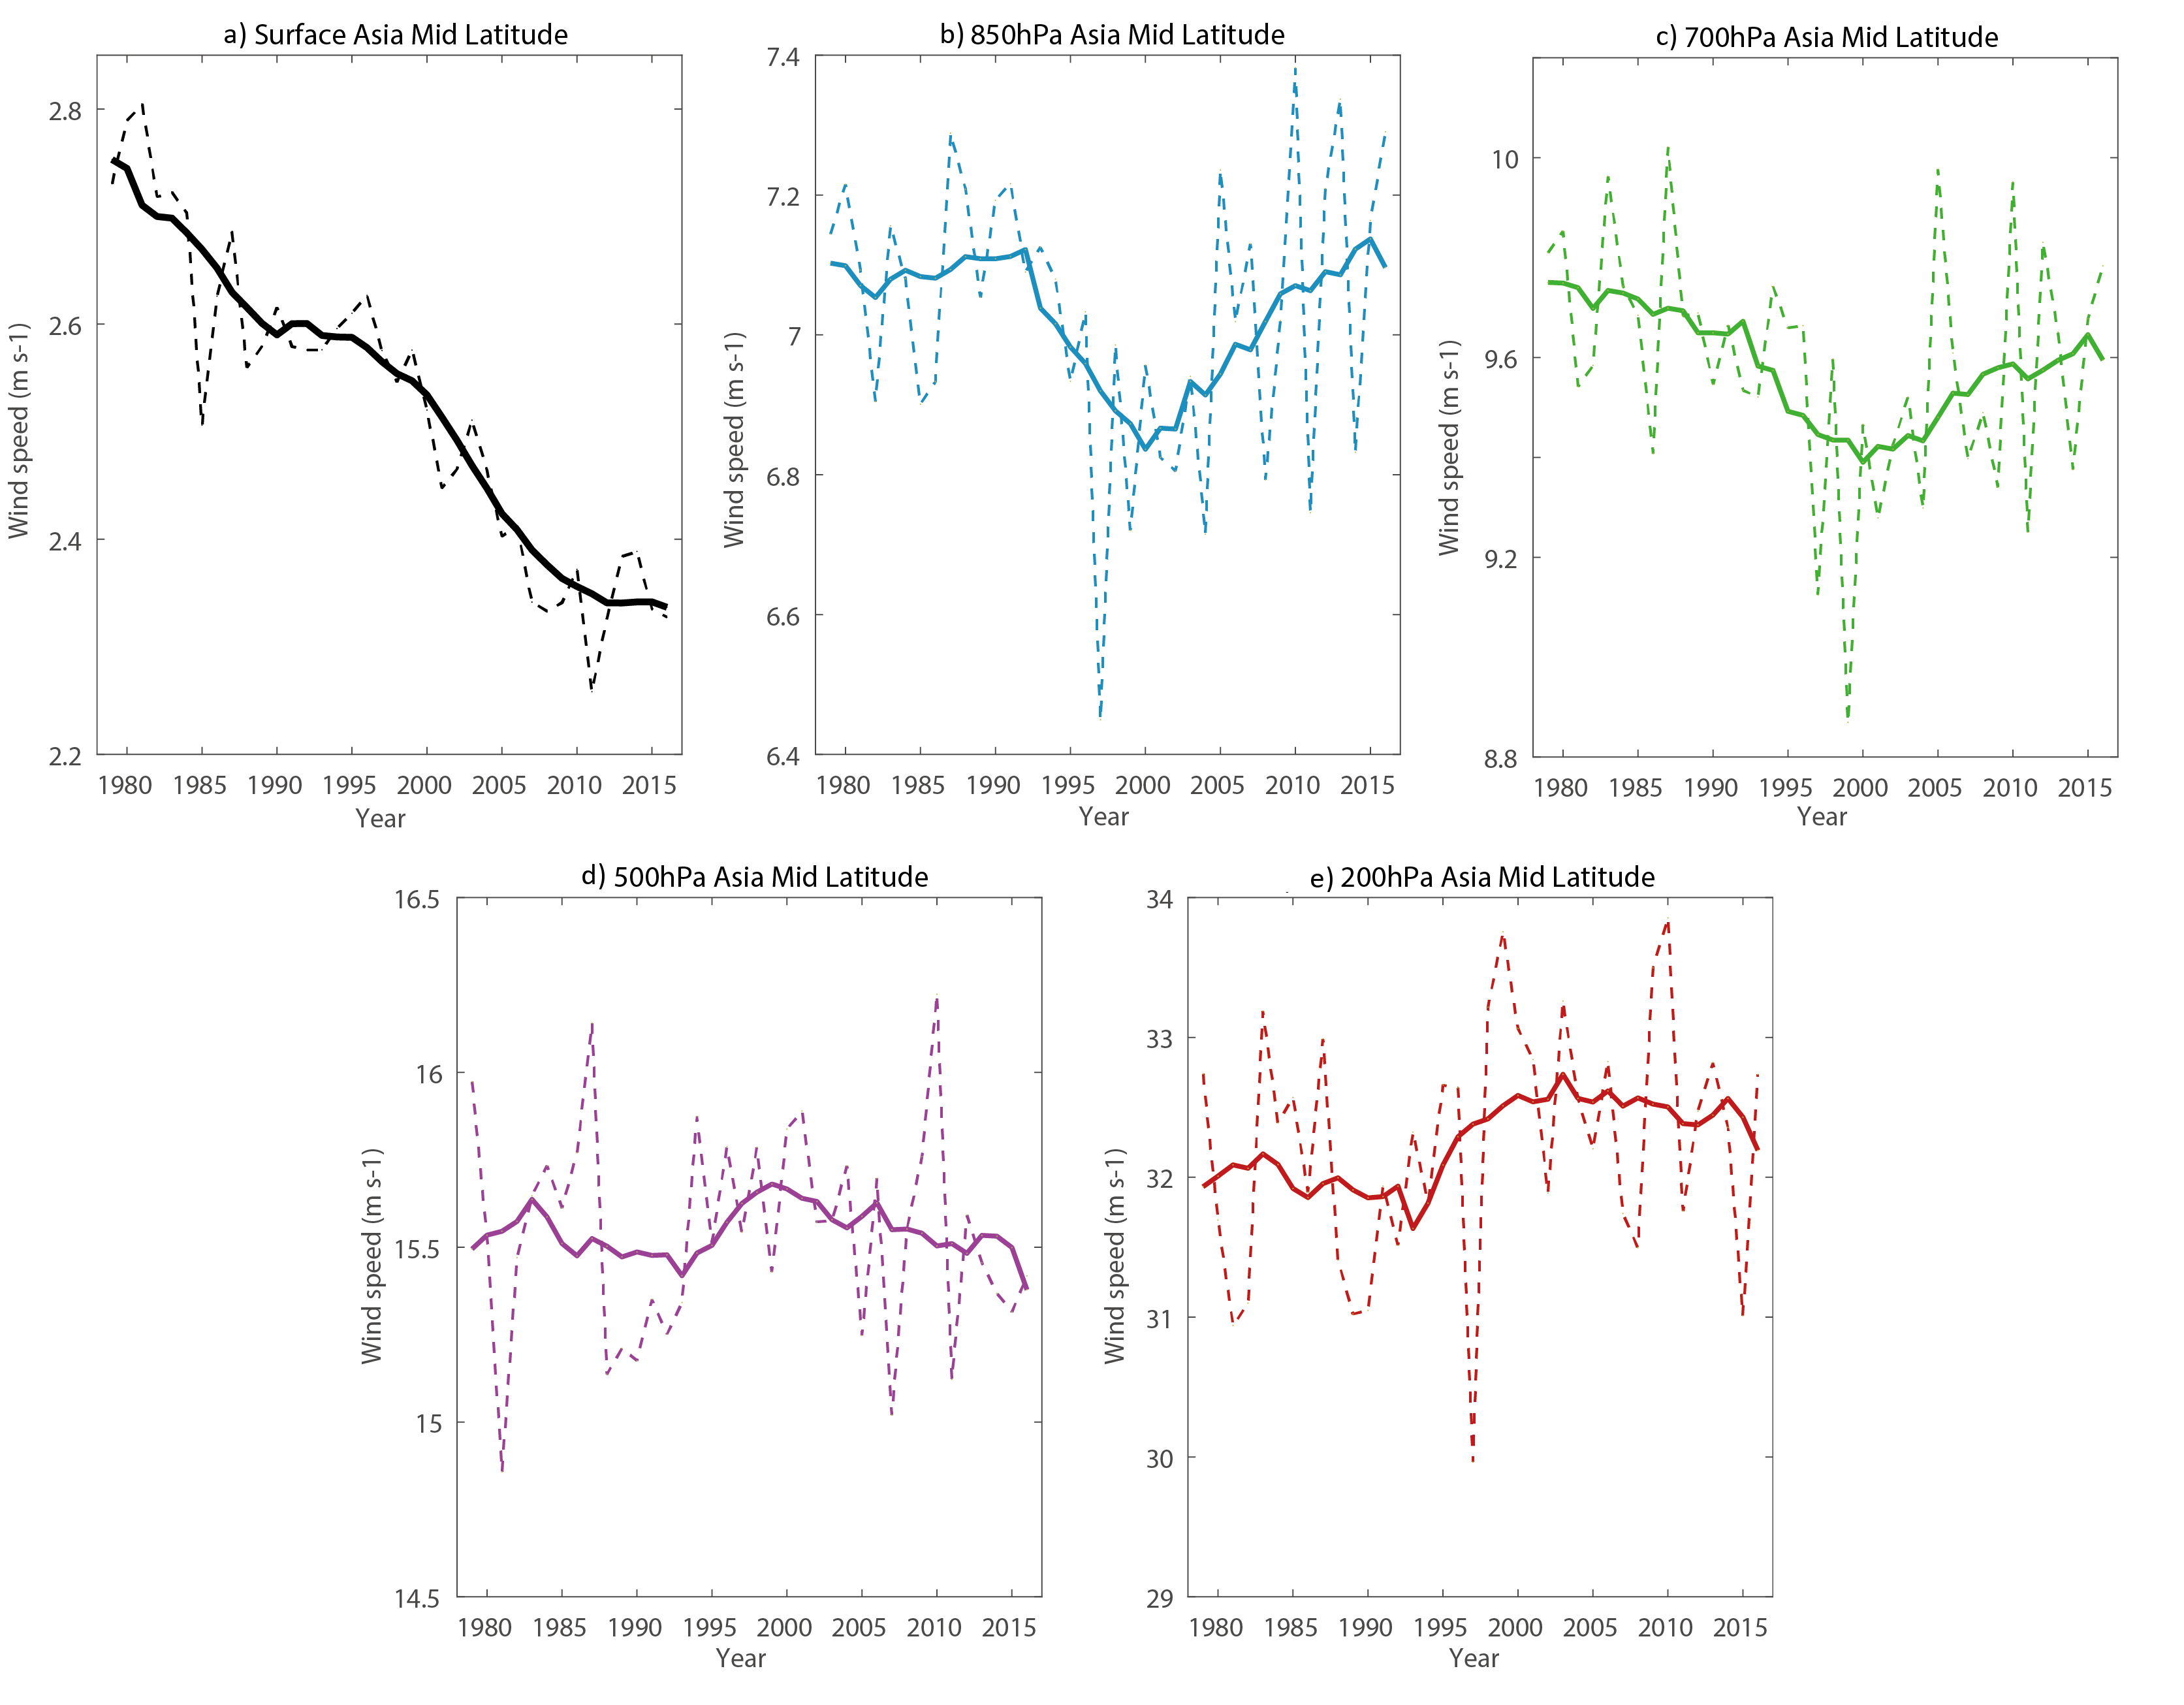
\includegraphics[width=0.85\textwidth]{亚洲中纬度对流层中位数风速演变}
    \bicaption{亚洲中纬度(20 - 55 N)对流层中位数风速演变($m ~ s^{-1}$)。与图 \ref{fig:globaltroposhereevolution}类似。}{Asian mid latitude (20 - 55 N) median troposhere wind speed evolution (in $m ~ s^{-1}$). Same as \ref{fig:globaltroposhereevolution}, but for Asia mid latitude}
    \label{fig:ASmidtroposhereevolution}
\end{figure}

\section{气压场变化的影响}

\begin{figure}[!b]
    \centering
    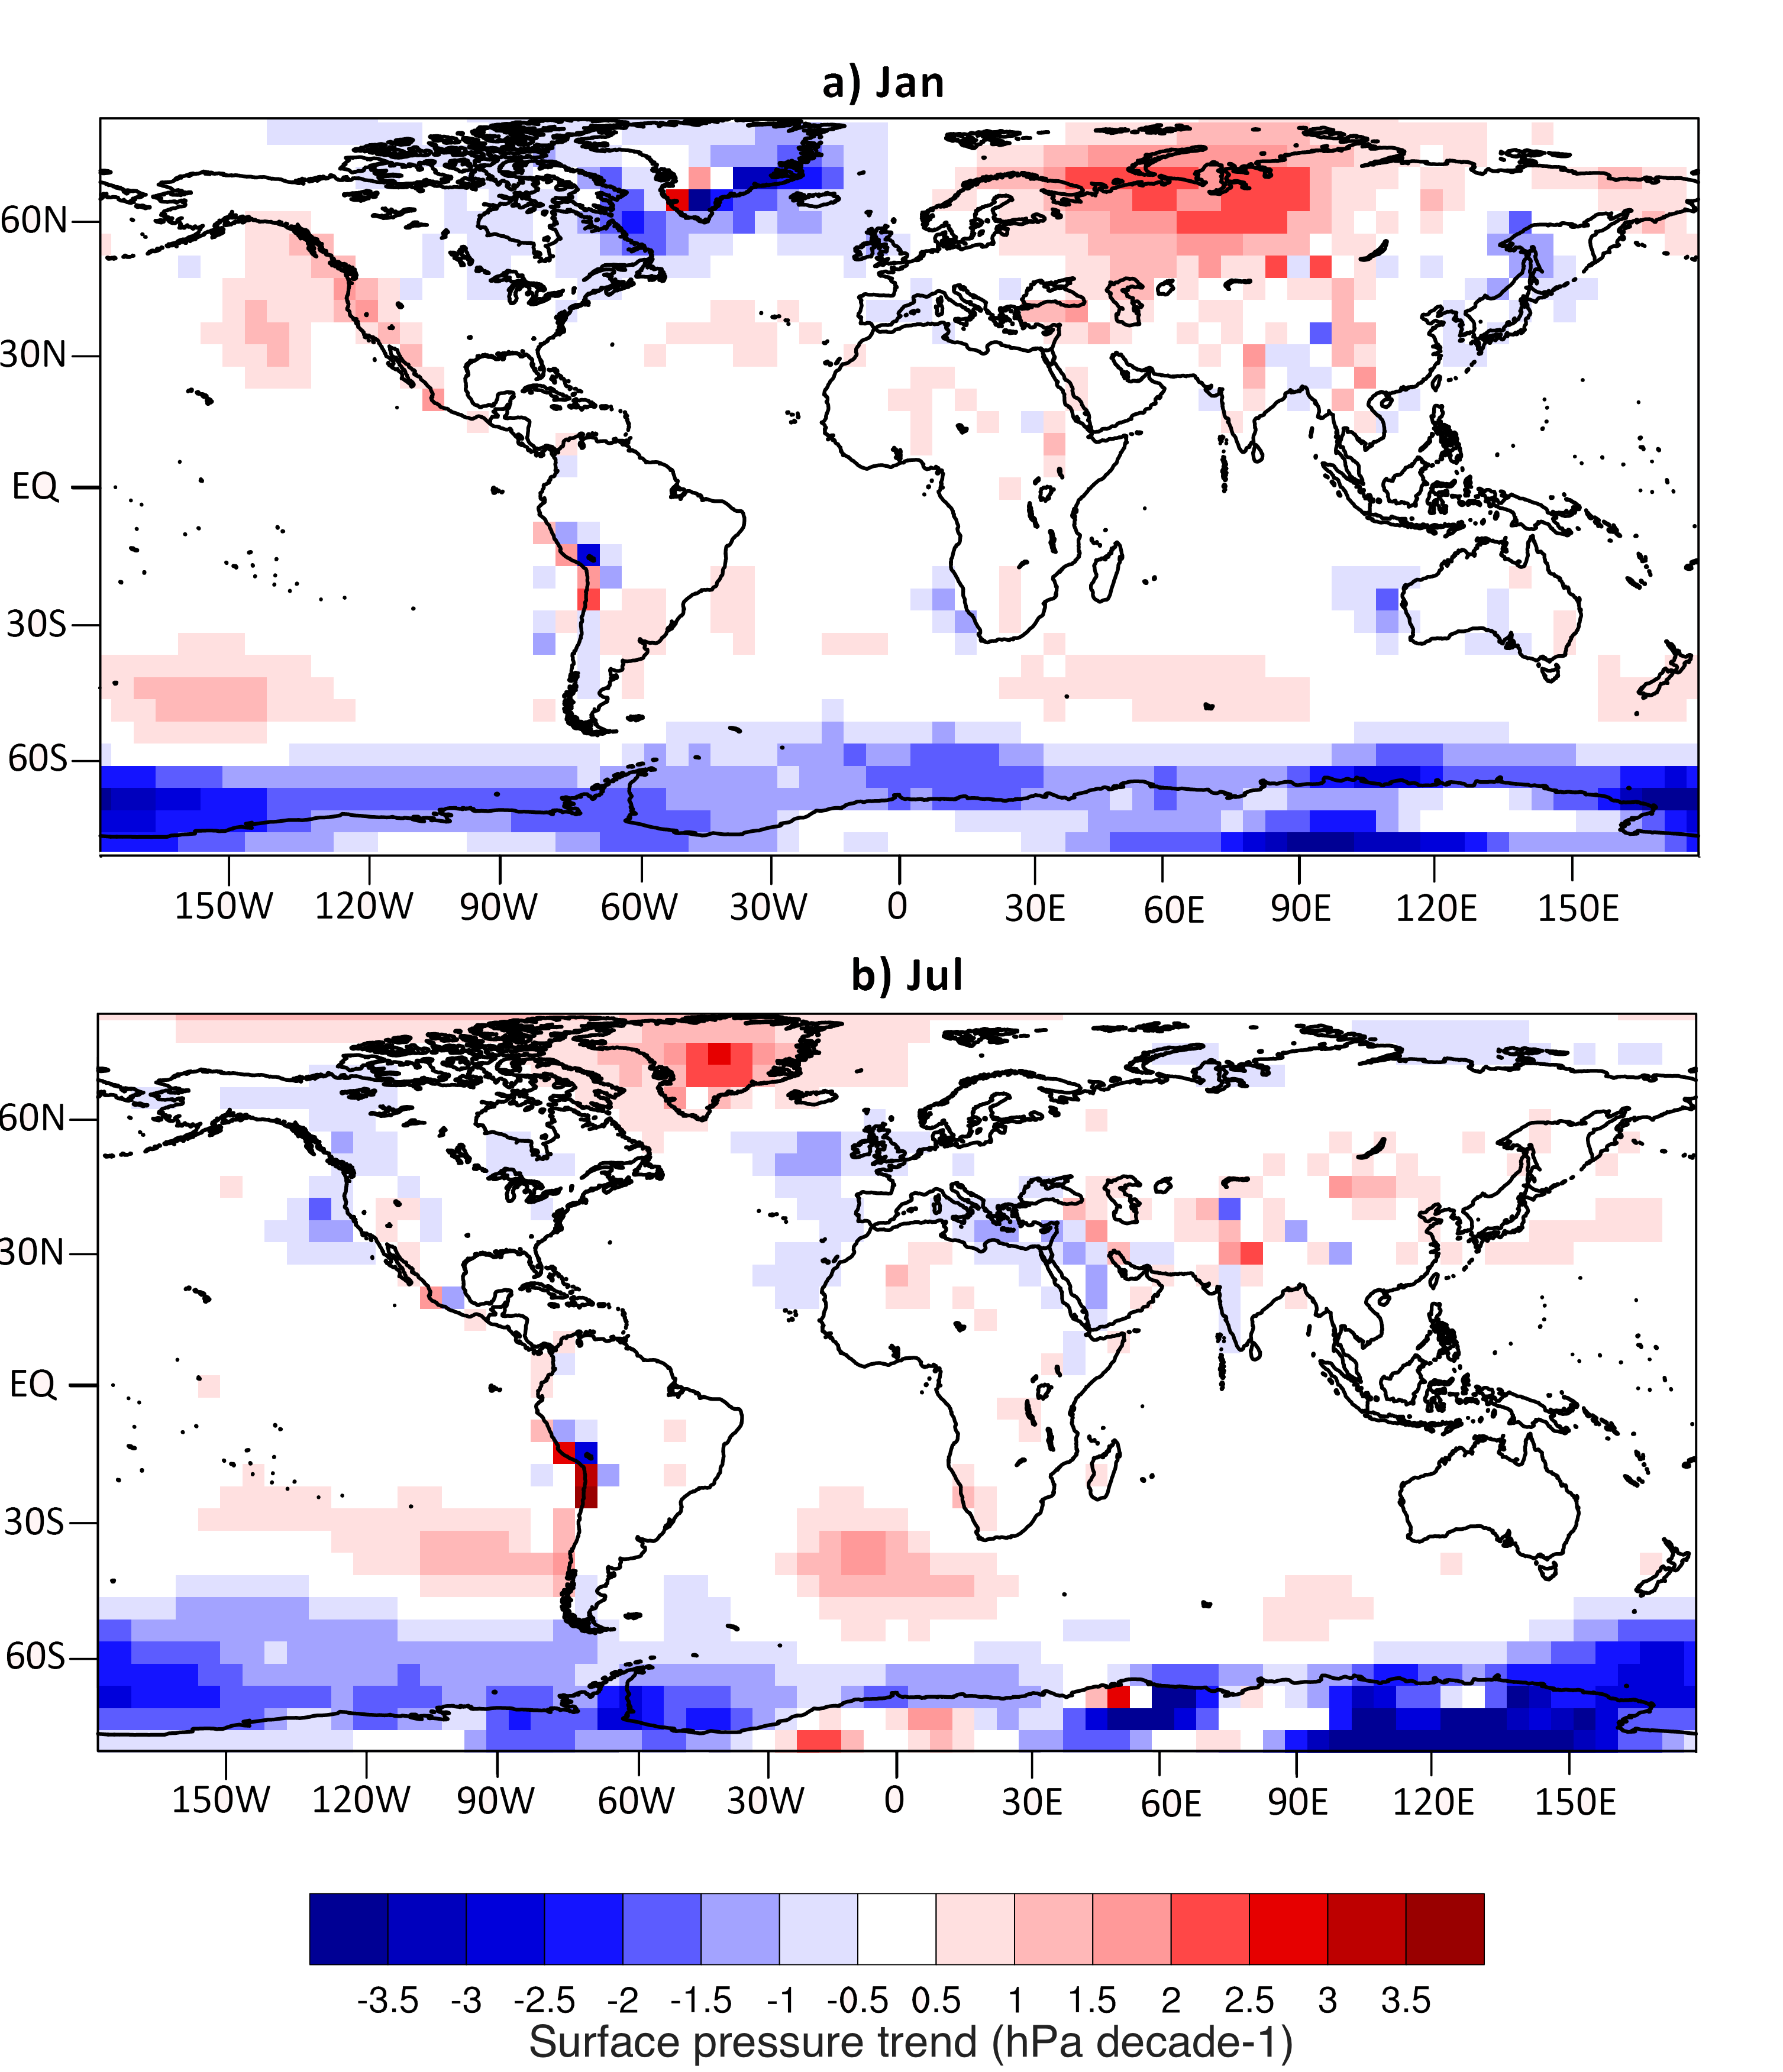
\includegraphics[width=0.8\textwidth]{海平面气压变化}
    \bicaption{海平面气压变化(hPa每十年)。a)一月海平面气压趋势,b)七月海平面气压趋势。}{Change in sea level pressure (in $ hPa ~ decade^{-1}$). a)Trend in January, b)Trend in July. }
    \label{fig:SLPchange}
\end{figure}

1月份海平面气压场的变化主要体现为冰岛低压和西伯利亚高压北部的增强,以及阿留申低压东部的减弱(图 \ref{fig:SLPchange} a))。其中冰岛低压增强会使得北大西洋风暴轴向北偏移,使得欧洲南部风速减小,北部风速增加 \citep{lifland2003the}。而西伯利亚高压北部增强配合日本以北气压下降使得冬季冷空气更容易侵入东亚,这也解释了为何亚洲冬季风速减弱慢于其他季节(第\ref{chap:SpatiotemporalCharacteristics}章 图 \ref{fig:regionalmedianwindtrend})。阿留申低压东南部减弱(即阿留申低压向西北偏移)会使得北太平洋风暴轴向北偏移,造成北美中低纬度风速减小\citep{任雪娟2007北太平洋风暴轴的变异特征及其与中纬度海气耦合关系分析},同时北美风速也会因为冰岛低压增强在北美形成异常偏南气流使得北极冷空气更不容易南下而减小。7月份海平面气压场的变化主要表现为冰岛低压的减弱(图 \ref{fig:SLPchange} b))。冰岛低压的减弱会使得北大西洋风暴轴向南偏移,使得欧洲南部风速增加,北部风速减小。如前文所述,1月份的情况与此刚好相反。这也解释了为何欧洲南部夏季风速减弱明显慢于冬季(第\ref{chap:SpatiotemporalCharacteristics}章 图 \ref{fig:EUwindtrend})。

\section{大尺度海温和环流系统变化的影响}

将北美洲、欧洲、亚洲中纬度和低纬度中位数风速分别与海表温度(SST)做相关,发现它们分别与一些海区SST相关性较高,下面逐个进行分析。

\begin{figure}[!htbp]
    \centering
    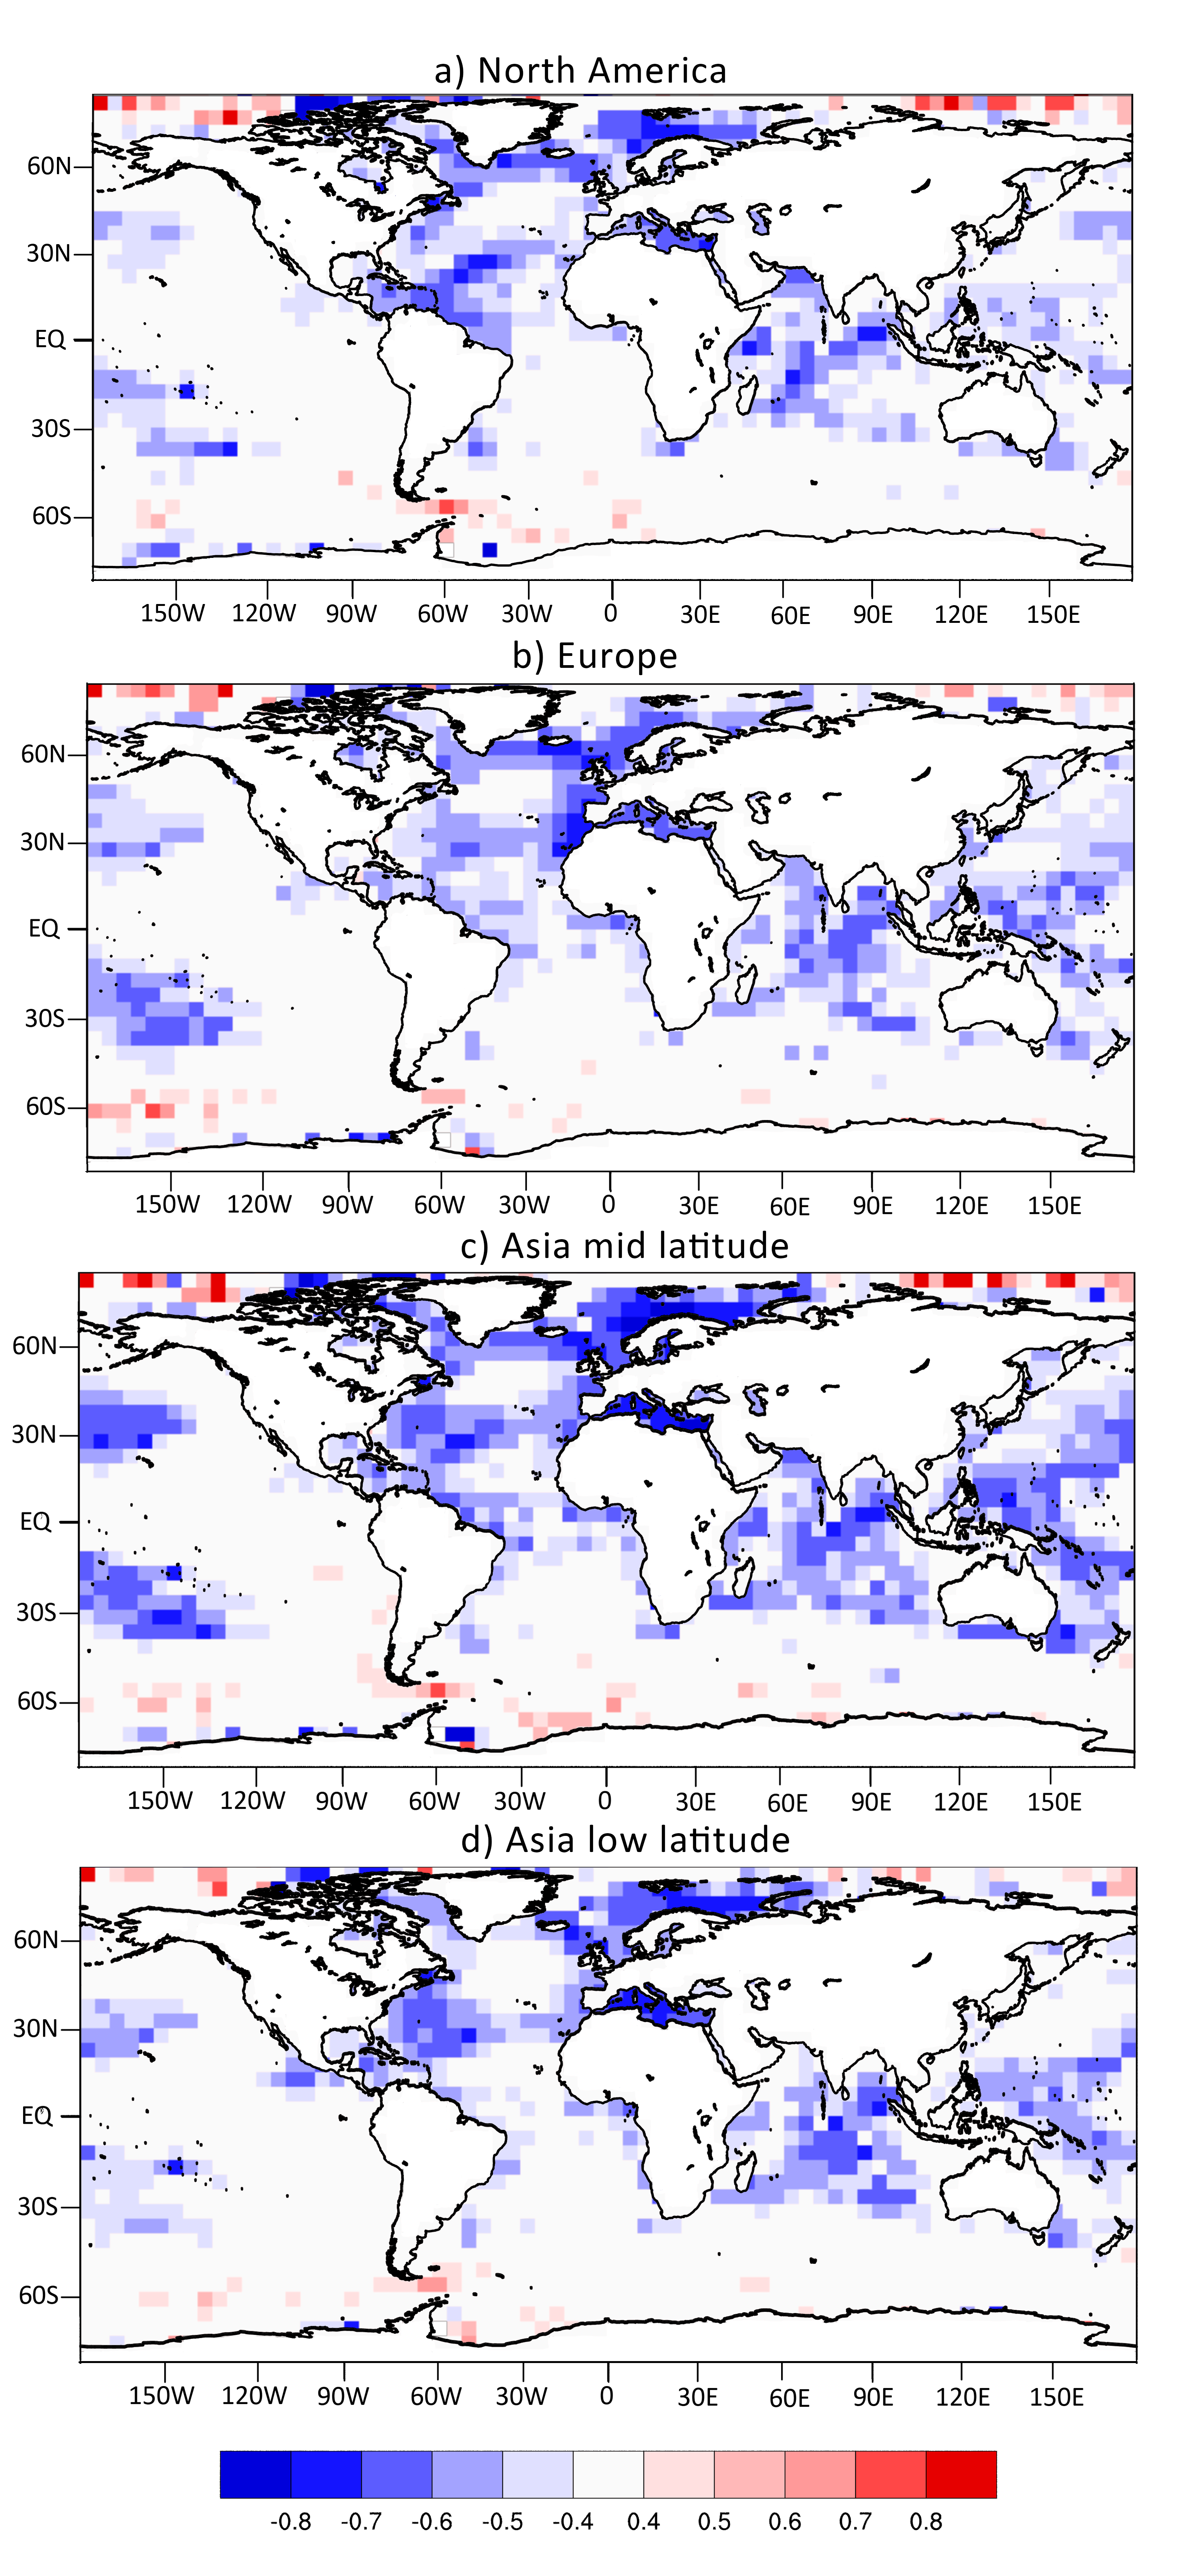
\includegraphics[width=0.63\textwidth]{风速与海温相关系数}
    \bicaption{ 地表风速与海温相关系数。a)北美洲,b)欧洲,c)亚洲中纬度(20 - 55 N)和d)亚洲低纬度(0 - 20 N)中位数风速与海温相关。相关系数0.4对应 p = 0.01}{Correlation coefficient between surface wind speed and SST. Correlation coefficient between median wind speed of a)North America, b)Europe, c)Asia mid latitude (20 - 55 N), d)Asia low latitude (0 - 20 N) and SST. Correlation coefficient of 0.4 corresponds to p = 0.01.}
    \label{fig:windspeedcorrSST}
\end{figure}

北美洲风速与附近的热带北大西洋以及北大西洋高纬海区SST有显著相关关系(图 \ref{fig:windspeedcorrSST} a))。其中,热带北大西洋海温变化可以由热带北大西洋指数(TNA)来表示,对比北美洲中位数风速和TNA的年代际变化,发现二者有相当好的对应关系(r = -0.95, p < 0.01),1987年前二者均较为平稳,1990-2010 北美洲风速持续下降,而TNA指数持续上升,2010年后二者又都回归平稳(图 \ref{fig:NAwindspeedTNA})。有研究表明,TNA正位相会使得中纬度到热带大气低层形成异常的偏北风,此异常风与北美洲中纬度气候态偏南风相反,从而对北美中纬度实际风速产生减弱的效果\citep{wang2002atlantic}。而北美风速与北大西洋高纬海区SST相关则预示着它可能与NAO存在联系。NAO强年冬季北美东部会出现较强的西南气流,阻止北极的冷空气南下,从而使北美东部风速减小。不过这种影响不是非常显著,因而NAO与北美风速没有体现很好的相关关系。

\begin{figure}[!t]
    \centering
    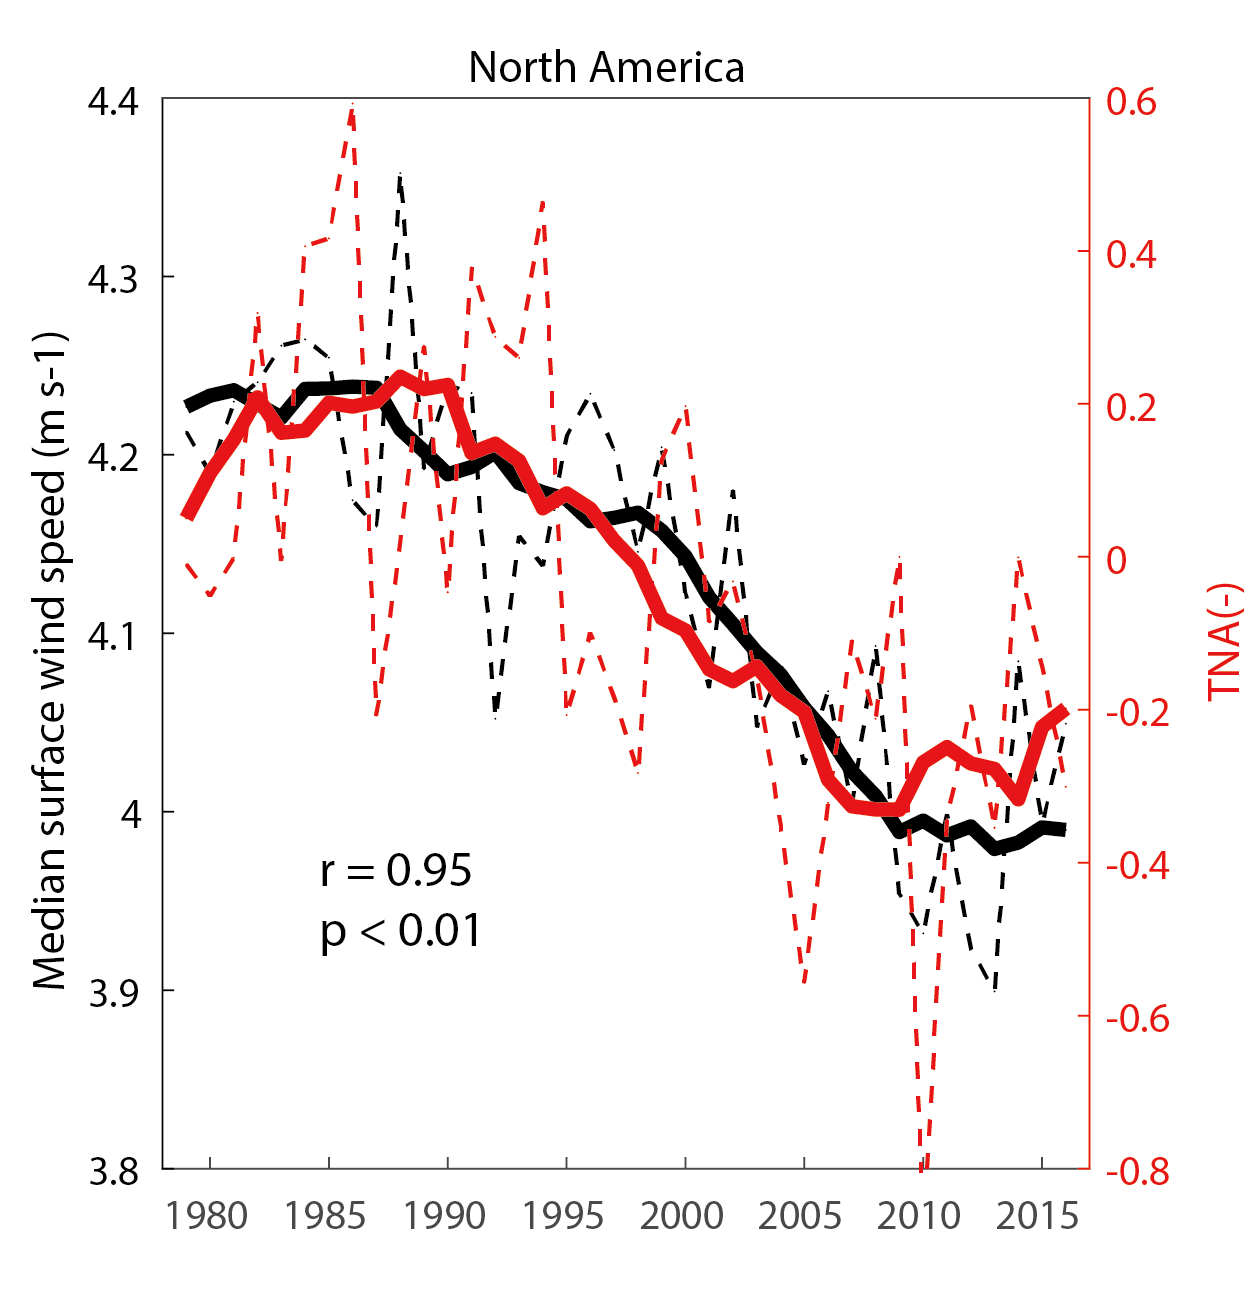
\includegraphics[width=0.45\textwidth]{北美风速与TNA}
    \bicaption{ 北美风速与TNA指数演变。黑色(红色)虚线为北美洲中位数风速(TNA指数年平均值),实线为虚线9年滑动平均结果,两实线的相关系数为0.95,p < 0.01。}{Evolution of North American wind speed and PDO index. Black (red) dash line is North American annual median wind speed (annual mean value of TNA index), solid line is 9-point moving mean of dash line, correlation coefficient between two solid lines is 0.95, p < 0.01.}
    \label{fig:NAwindspeedTNA}
\end{figure}

欧洲风速与北大西洋高纬海温有显著相关,预示着它可能与NAO存在关联(图 \ref{fig:windspeedcorrSST} b))。将去趋势的欧洲中位数风速序列与NAO指数对比发现,二者有显著相关,相关系数达到 -0.48(p < 0.01)(图 \ref{fig:EUwindspeedNAO})。之前已有许多研究发现NAO与欧洲风速的相关关系\citep{beniston2005mountain, earl20131980–2010, zeng2019a}。目前普遍认为,NAO对欧洲风速的影响通过以下过程进行:NAO的强弱会影响北大西洋上空急流的位置,而急流位置的改变又会使风暴轴发生偏移,当NAO处于正位相是,风暴轴偏北,使得气旋在欧洲活动的位置偏北,最终造成欧洲南部风速偏小,而北部偏大,NAO处于负位相时刚好相反\citep{lifland2003the, zeng2019a}。由于研究所用到的站点位于欧洲北部的较少,所以NAO对于欧洲南部的影响会主导分析的结果。

\begin{figure}[!b]
    \centering
    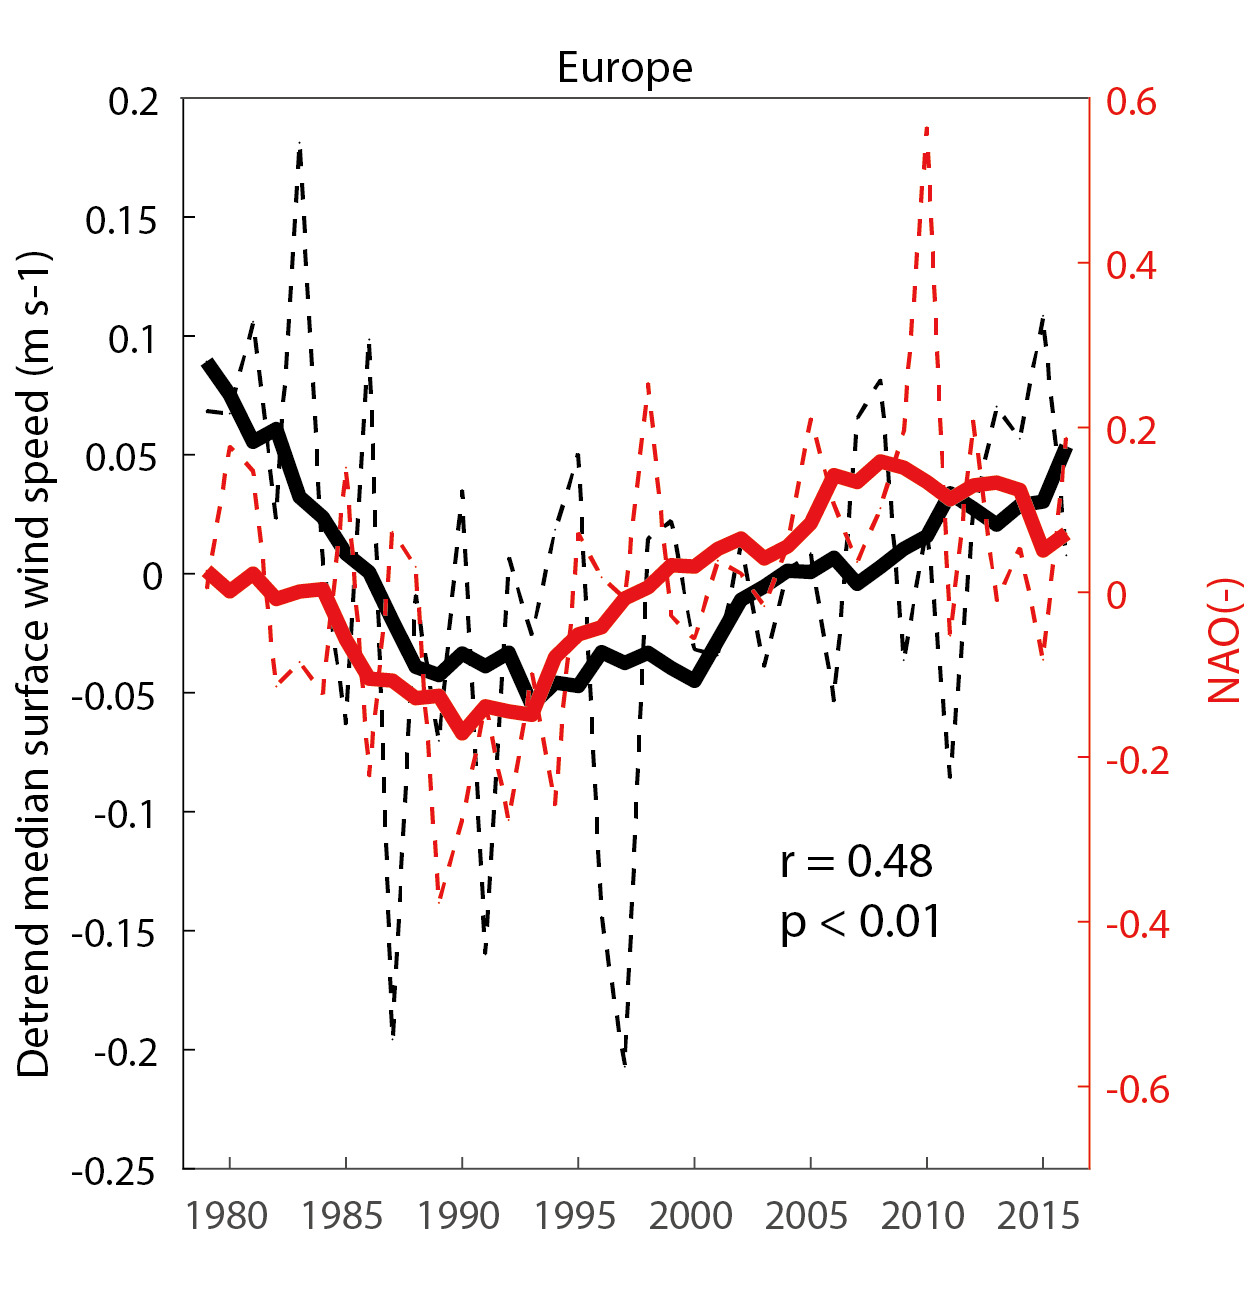
\includegraphics[width=0.45\textwidth]{欧洲风速与NAO}
    \bicaption{ 欧洲风速与NAO指数演变。黑色(红色)虚线为欧洲中位数风速(NAO指数年平均值),实线为虚线9年滑动平均结果,两实线的相关系数为0.48,p < 0.01。}{Evolution of European wind speed and NAO index. Black (red) dash line is European annual median wind speed (annual mean value of NAO index), solid line is 9-point moving mean of dash line, correlation coefficient between two solid lines is 0.48, p < 0.01.}
    \label{fig:EUwindspeedNAO}
\end{figure}

亚洲低纬度风速与印度洋海温有较强的相关(图 \ref{fig:windspeedcorrSST} d))。\citet{yang2010linking}发现,印度洋偶极子模态(IOB)会使得印度冬季风减弱,从使亚洲低纬度陆地地表风速减小。近期有许多研究表明,南亚季风出现了减弱的现象\citep{bollasina2011anthropogenic, sooraj2015global},印度洋海温变化或许在其中起到了一定作用。

亚洲中纬度风速与中纬度北太平洋、中纬度南太平洋和西太平洋以及印度洋海温有较强相关(图 \ref{fig:windspeedcorrSST} c))。其中它与中纬度北太平和中纬度南太平相关预示着于PDO之间的联系。PDO负位相会产生异常的东风,与中纬度盛行的西风相抵消,从而使亚洲中纬度风速减小\citep{zeng2019a}。此外,西太平洋暖池区也与亚洲中纬度风速有很好的负相关,其中的关联在于夏季西太平洋暖池增温速度快于东亚大陆,海陆热力对比减小从而减弱了东亚夏季风,造成亚洲中纬度风速减小\citep{xu2006steady}。将PDO指数与去趋势的西太平洋暖池面积指数作为回归量回归到去趋势的亚洲中纬度风速序列,发现有一定的相关性(图 \ref{fig:ASwindspeedPDOandWPWPA})。印度洋海温影响亚洲中纬度风速的方式应与其影响亚洲低纬度类似,但影响可能并不显著。

\begin{figure}[!b]
    \centering
    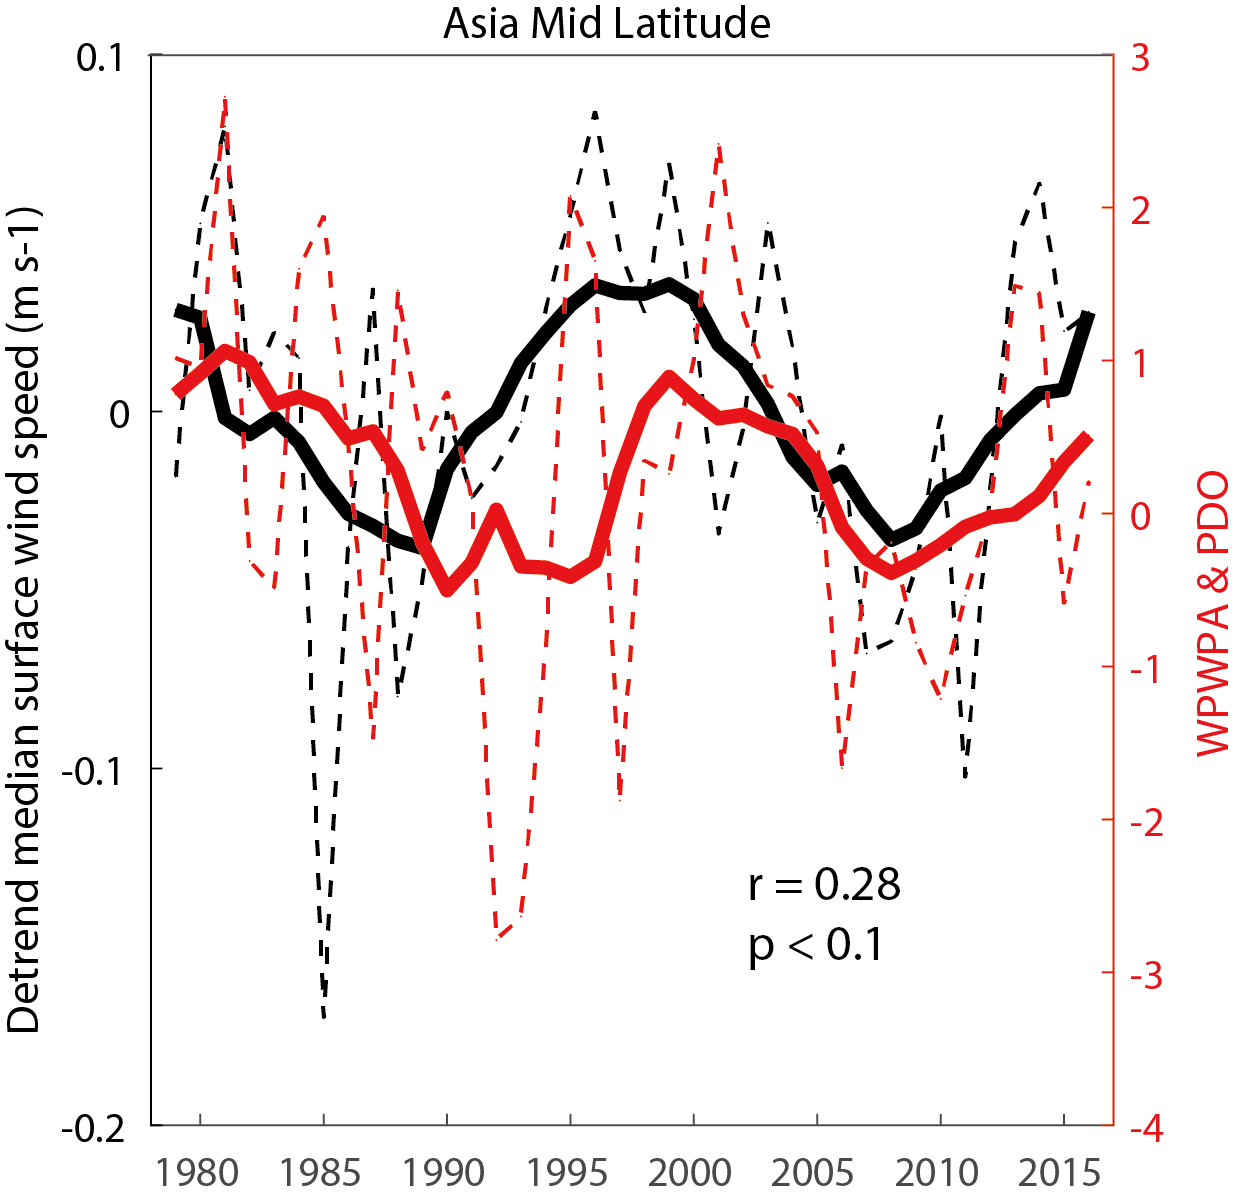
\includegraphics[width=0.45\textwidth]{亚洲中纬度风速与WPWPA和PDO}
    \bicaption{ 亚洲中纬度风速与西太平洋暖池面积指数(WPWPA)和PDO指数演变。黑色(红色)虚线为亚洲中纬度地区中位数风速(PDO指数年均值 $\times$-0.88 $+$ 去趋势WPWPA指数年均值 $\times$ -1.44),实线为虚线9年滑动平均结果,两实线的相关系数为0.28,p < 0.1。}{Evolution of Asian mid latitude wind speed, WPWPA index and PDO index. Black (red) dash line is Asian mid latitude annual median wind speed (annual mean value of PDO index $\times$ -0.88 $ + $ detrend annual mean value of WPWPA index $\times$ -1.44 ), solid line is 9-point moving mean of dash line, correlation coefficient between two solid lines is 0.28, p < 0.1.}
    \label{fig:ASwindspeedPDOandWPWPA}
\end{figure}

\section{本章小结}

本章从大气运动驱动力的变化出发,分析了对流层风速的变化,气压场变化,大尺度海温和环流系统对于陆地地表风速的影响,得到以下主要结论:

\begin{enumerate}

\item 在欧洲和亚洲中纬度地区,对流层低层风速都出现了下降,因而这两个地区地表风速下降可以由高空风速下降部分解释,但高空风速下降的速度远小于地表,因而高空风速变化不是地表风速下降的主要原因。而在北美洲和亚洲低纬度地区,对流层低层风速都出现了上升,尤其是北美洲,几乎所有探空站点都表现出风速上升,因而这两个地区地表风速下降难以由高空风速变化解释。无论在在北美洲、欧洲、亚洲低纬度和中纬度地区,地表与高层风速年代际变化均没有表现出很好的一致性。

\item 1月海平面气压场变化主要表现为冰岛低压减弱、西伯利亚高压北部增强和阿留申低压向西北偏移,会使得南欧和北美风速减小,而北欧和亚洲风速增加。7月海平面气压场变化主要表现为冰岛低压增强,会使得南欧风速增加而北欧风速减小。

\item 北美洲和欧洲陆地地表风速年代际变化分别受到TNA和NAO的显著影响,亚洲中纬度陆地地表风速年代际变化受到PDO和西太平洋暖池面积的共同影响。

\end{enumerate}